	\documentclass[a4paper,12pt]{article} 

\usepackage[unicode, pdftex]{hyperref}

% новая команда \RNumb для вывода римских цифр
\newcommand{\RNumb}[1]{\uppercase\expandafter{\romannumeral #1\relax}}

%Добавляет возможность искать и копировать текст
\usepackage{cmap}

%Убирает пробел между названием таблицы/рисунка и самой таблицей/рисунком
\usepackage{caption}
\captionsetup[table]{skip= -0 cm}
\captionsetup[figure]{skip= -0 cm}

%Выравнивание названия таблиц по левому краю
%\usepackage[nooneline]{caption} 
%Размеры отступов 
\usepackage[left=20mm, top=20mm, right=20mm, bottom=20mm, footskip=10mm]{geometry}

%Рисунки
\usepackage{graphicx}
\usepackage{wrapfig} %обтекание элементов
\graphicspath{{graphs}{figures}}  % папки с картинками

%Русский язык в формулах
\usepackage{mathtext}

%  Русский язык
\usepackage[T2A]{fontenc}			
\usepackage[utf8]{inputenc}			
\usepackage[english,russian]{babel}	

%Красная строка для первого абзаца
\usepackage{indentfirst}

%Готические буквы
\usepackage{amssymb}

% Математика
\usepackage{amsmath,amsfonts,amssymb,amsthm,mathtools} 
\usepackage{wasysym}

%Цветные подписи в таблице
\usepackage[table,xcdraw]{xcolor}

%Сделать несколько рядов одним
\usepackage{multirow}

\usepackage{fancyhdr} % Колонтитулы
 	\pagestyle{fancy}
 	\renewcommand{\headrulewidth}{0.3mm}  % Толщина линейки, отчеркивающей верхний колонтитул
 	%\lfoot{Нижний левый}
 	%\rfoot{Нижний правый}
 	\rhead{Белостоцкий Артмемий, Б04-006}
 	%\chead{Верхний в центре}
 	\lhead{Лабораторная работа №5.1.1}
 	\renewcommand{\footrulewidth}{0.3mm}
 	\cfoot{\thepage} % По умолчанию здесь номер страницы
 	
 	
%\captionsetup[table]{
%  position=above,
%  justification=raggedright,
  %labelsep=newline, % <<< label and text on different lines
%  singlelinecheck=false % <<< raggadright also when the cap%tion is shorter
                        % than a single line
%}
 	
\begin{document} 

%Титульник 
\begin{titlepage}
	\begin{center}
		\large 	МИНИСТЕРСТВО ОБРАЗОВАНИЯ И НАУКИ РОССИЙСКОЙ ФЕДЕРАЦИИ\\
				МОСКОВСКИЙ ФИЗИКО-ТЕХНИЧЕСКИЙ ИНСТИТУТ \\
				(НАЦИОНАЛЬНЫЙ ИССЛЕДОВАТЕЛЬСКИЙ УНИВЕРСИТЕТ)\\ 
				ФИЗТЕХ-ШКОЛА ЭЛЕКТРОНИКИ, ФОТОНИКИ \\
				И МОЛЕКУЛЯРНОЙ ФИЗИКИ \\
		
		
		\vspace{4.0 cm}
		Лабораторная работа № 5.1.1 \\ 
		\LARGE \textbf{Фотоэффект}
	\end{center}
	\vspace{3 cm} \large
	
	\begin{flushright}
		выполнил студент 3 курса \\
		{группы Б04-006}\\
		\textbf{Белостоцкий Артемий}\\
	\end{flushright}
	
	\vfill

	\begin{center}
	Долгопрудный, 2022 г.
	\end{center}
\end{titlepage}                                                                      

\section*{Аннотация}
В данной работе будет исследована зависимость фототока от величины задерживающего потенциала и длины волны подающего излучения, что позволит оценить постоянную Планка. Также процесс градуировки, используемого в данной работе монохроматора, будет представлен.	 

\section*{Экспериментальная установка}

\begin{figure}[h!]
	\centering
	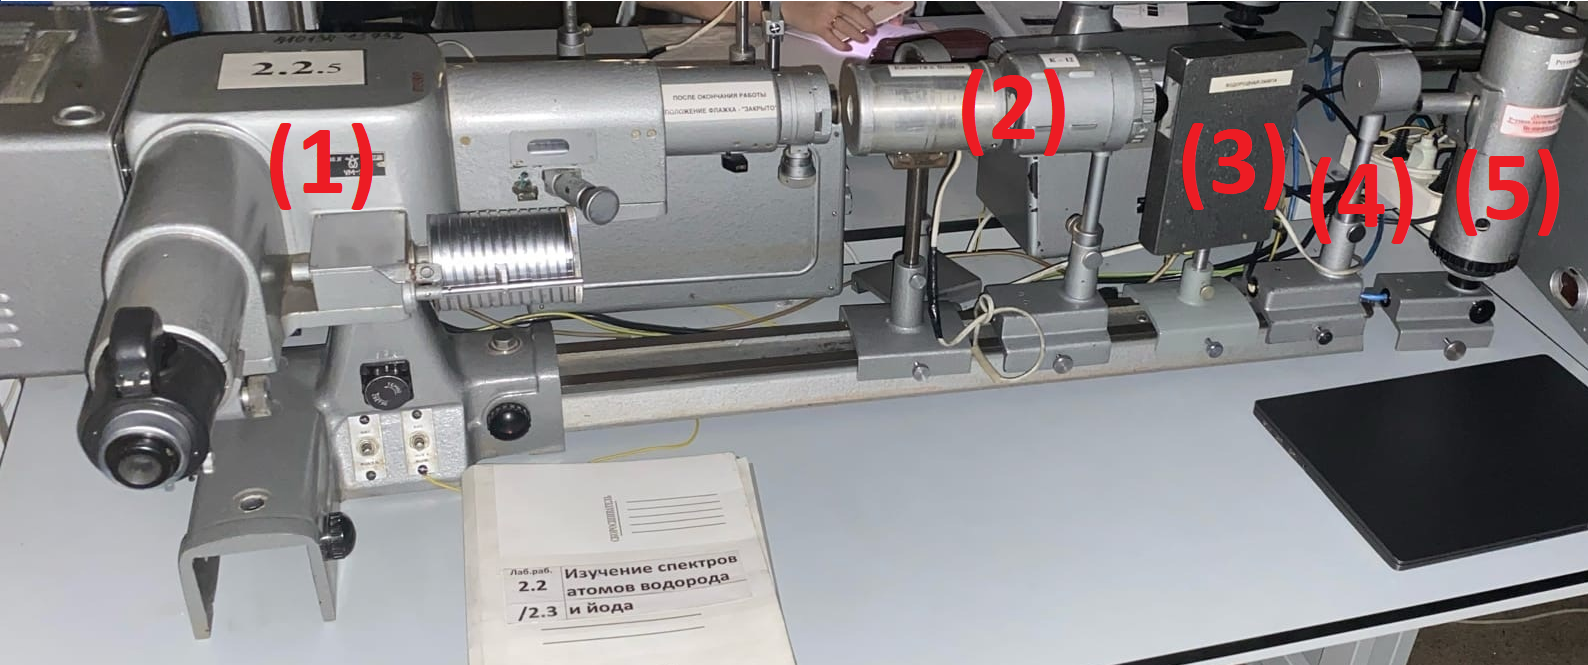
\includegraphics[width = \linewidth]{setup}
	\caption{Экспериментальная установка. (1) -- монохроматор, (2) -- пульт управления электроникой, (3) -- линза (коллиматор), (4) -- источник света, (5) -- вольтметры}
	\label{fig1:setup}
\end{figure}

\section*{Ход работы}

\subsubsection*{Калибровка монохроматора}

Используя окуляр и неоновую лампу, проградуируем барабан монохроматора, зная спектр неоновой лампы (Рис \ref{fig2:spectre} )

\pagebreak

\begin{figure}[h!]
	\centering
	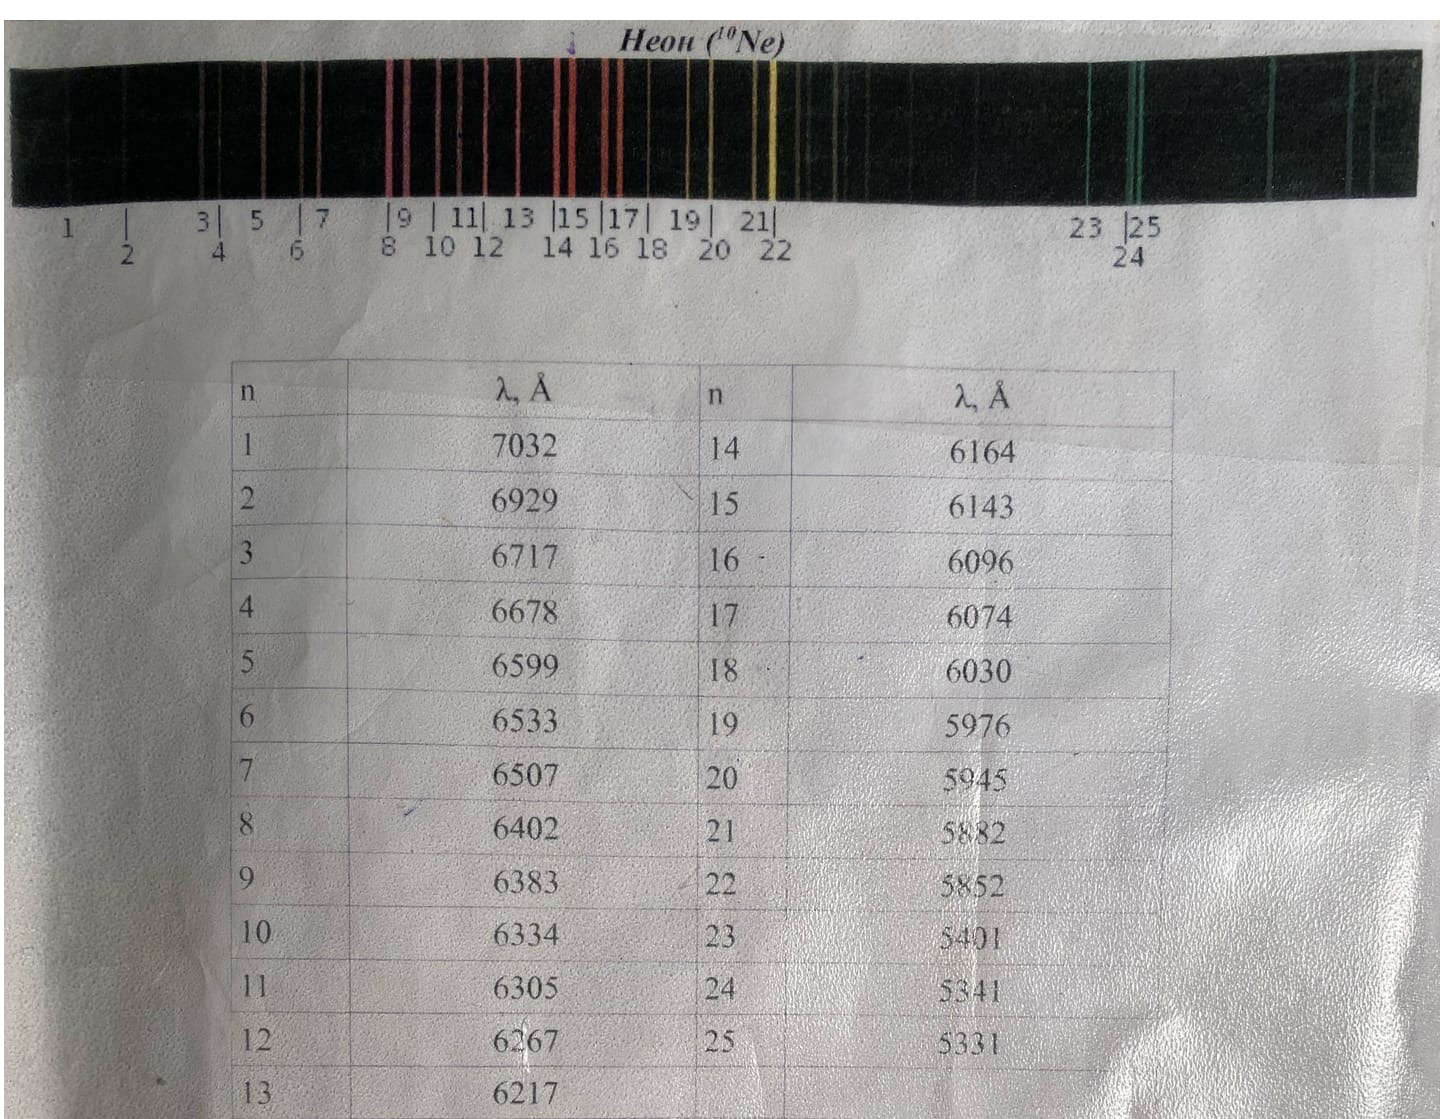
\includegraphics[width = 0.8\linewidth]{spectre}
	\caption{Спектральные линии неона и соответствующие им длины волн}
	\label{fig2:spectre}
\end{figure}

По полученным данным построим график зависимости угла, указываемого на барабане, от длины волны спектральной линии $Ne$.

\begin{figure}[h!]
	\centering
	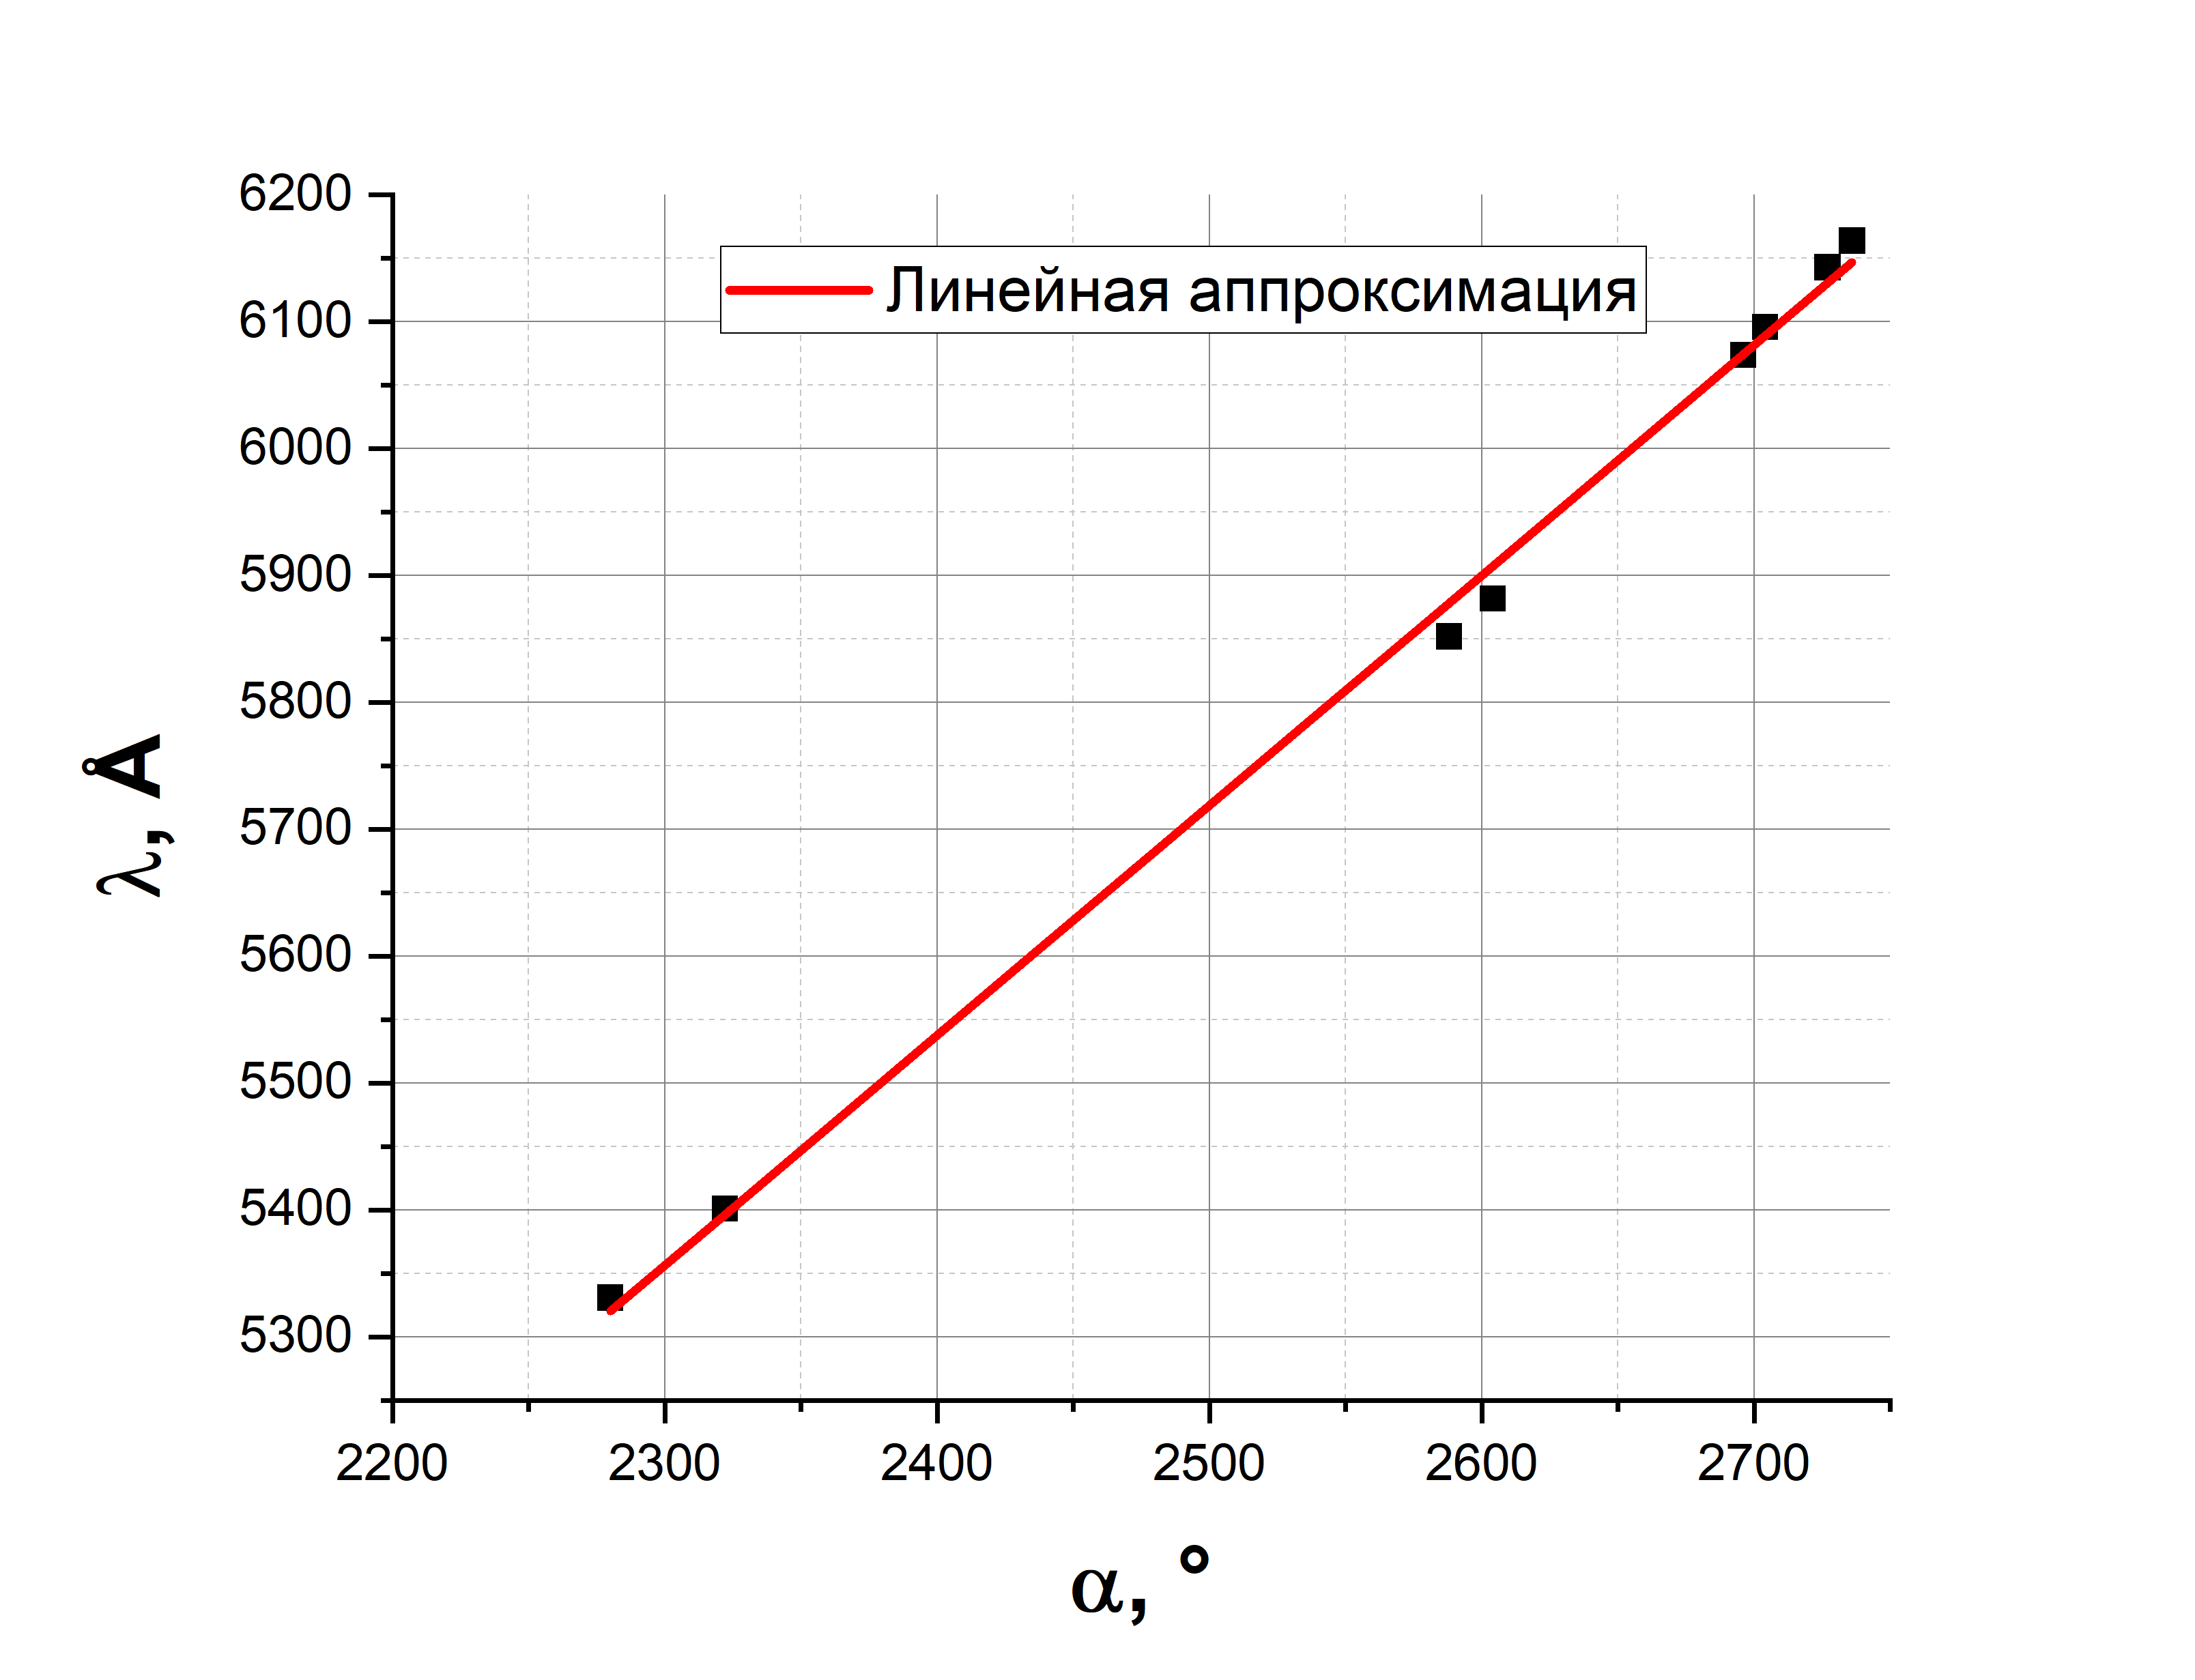
\includegraphics[width = 0.8\linewidth]{calibration_1}
	\caption{Калибровочный график зависимости угла, указанного на барабане монохроматора, от длины волны спектральной линии $Ne$}
	\label{graph1:calibration_1}
\end{figure}

\pagebreak

При дальнейших попытках провести измерения, оказалось, что пульт управления электроникой (2) (Рис \ref{fig2:spectre}) -- неисправен, поэтому пришлось проводить дальнейшие измерения на другой установке.

Так же откалибруем монохроматор на этой установке и приведем калибровочный график:

\begin{figure}[h!]
	\centering
	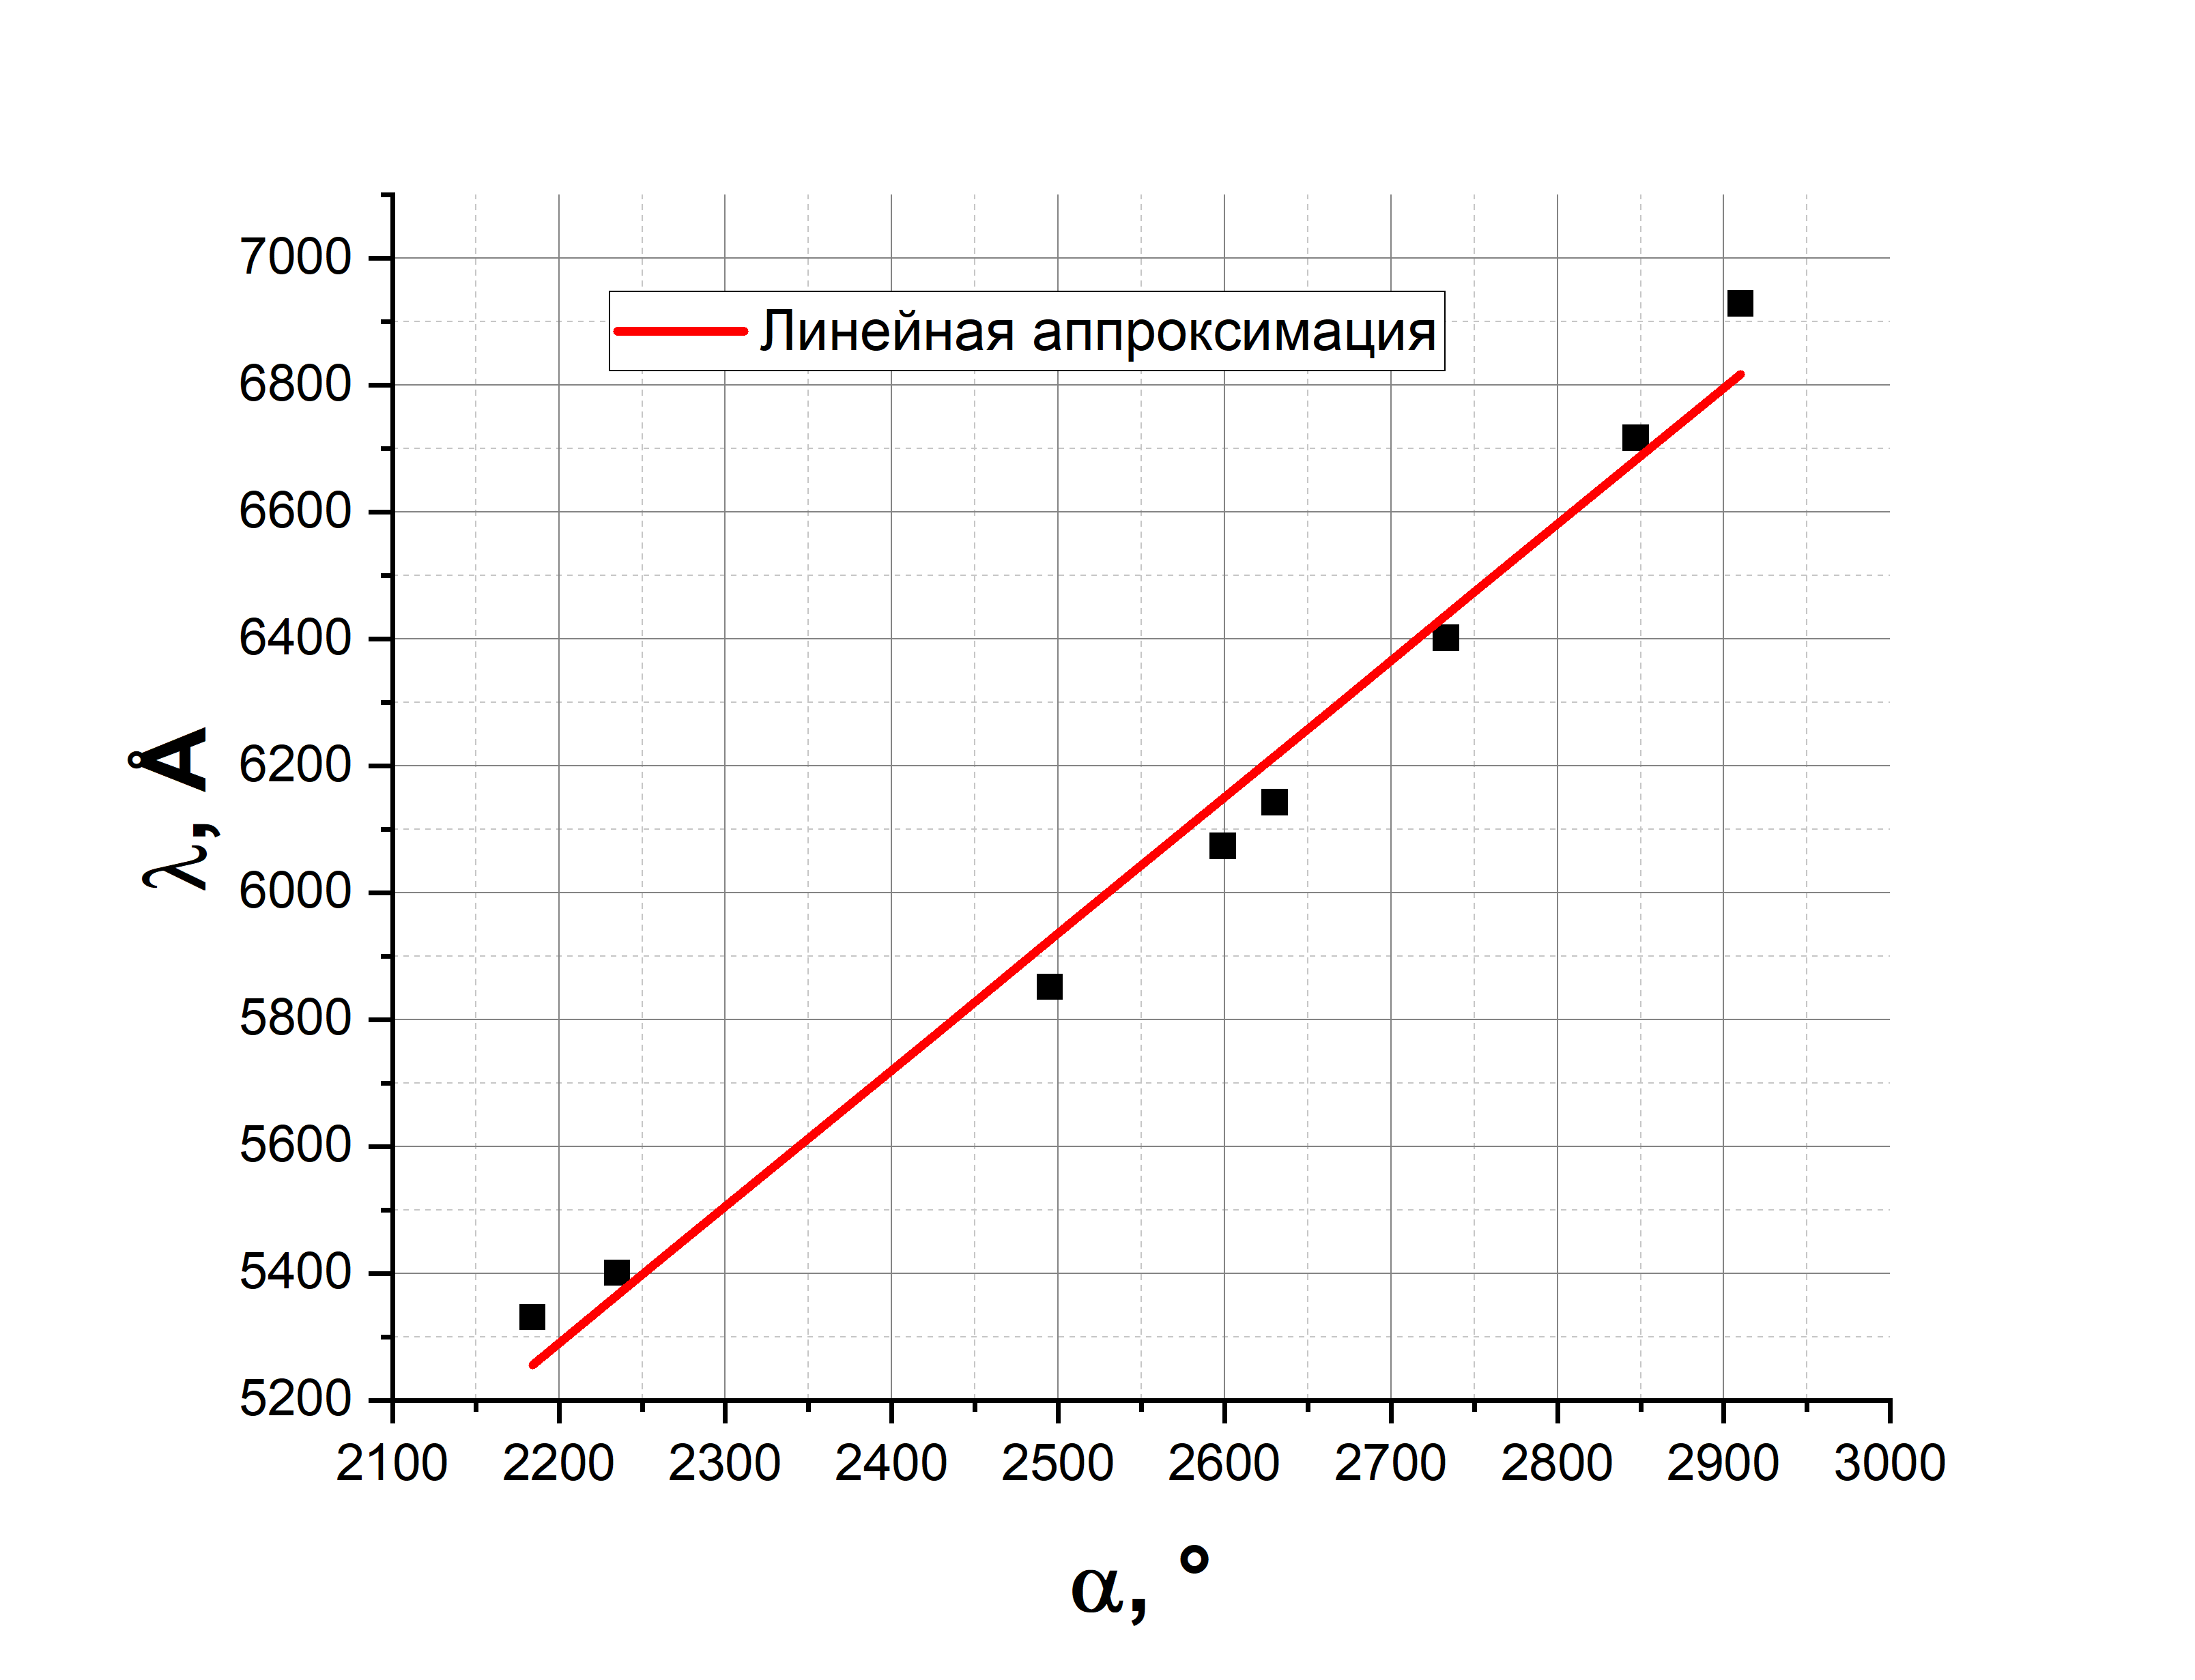
\includegraphics[width = \linewidth]{calibration_2}
	\caption{Калибровочный график зависимости угла, указанного на барабане монохроматора, от длины волны спектральной линии $Ne$}
	\label{graph2:calibration_2}
\end{figure}

Снимем зависимость фототока от напряжения для 4 различных значений длин волн. Построим серию графиков $\sqrt{I} = f(V)$ и для каждой длины волны определим запирающее напряжение.

\pagebreak

\begin{figure}[h!]
	\centering
	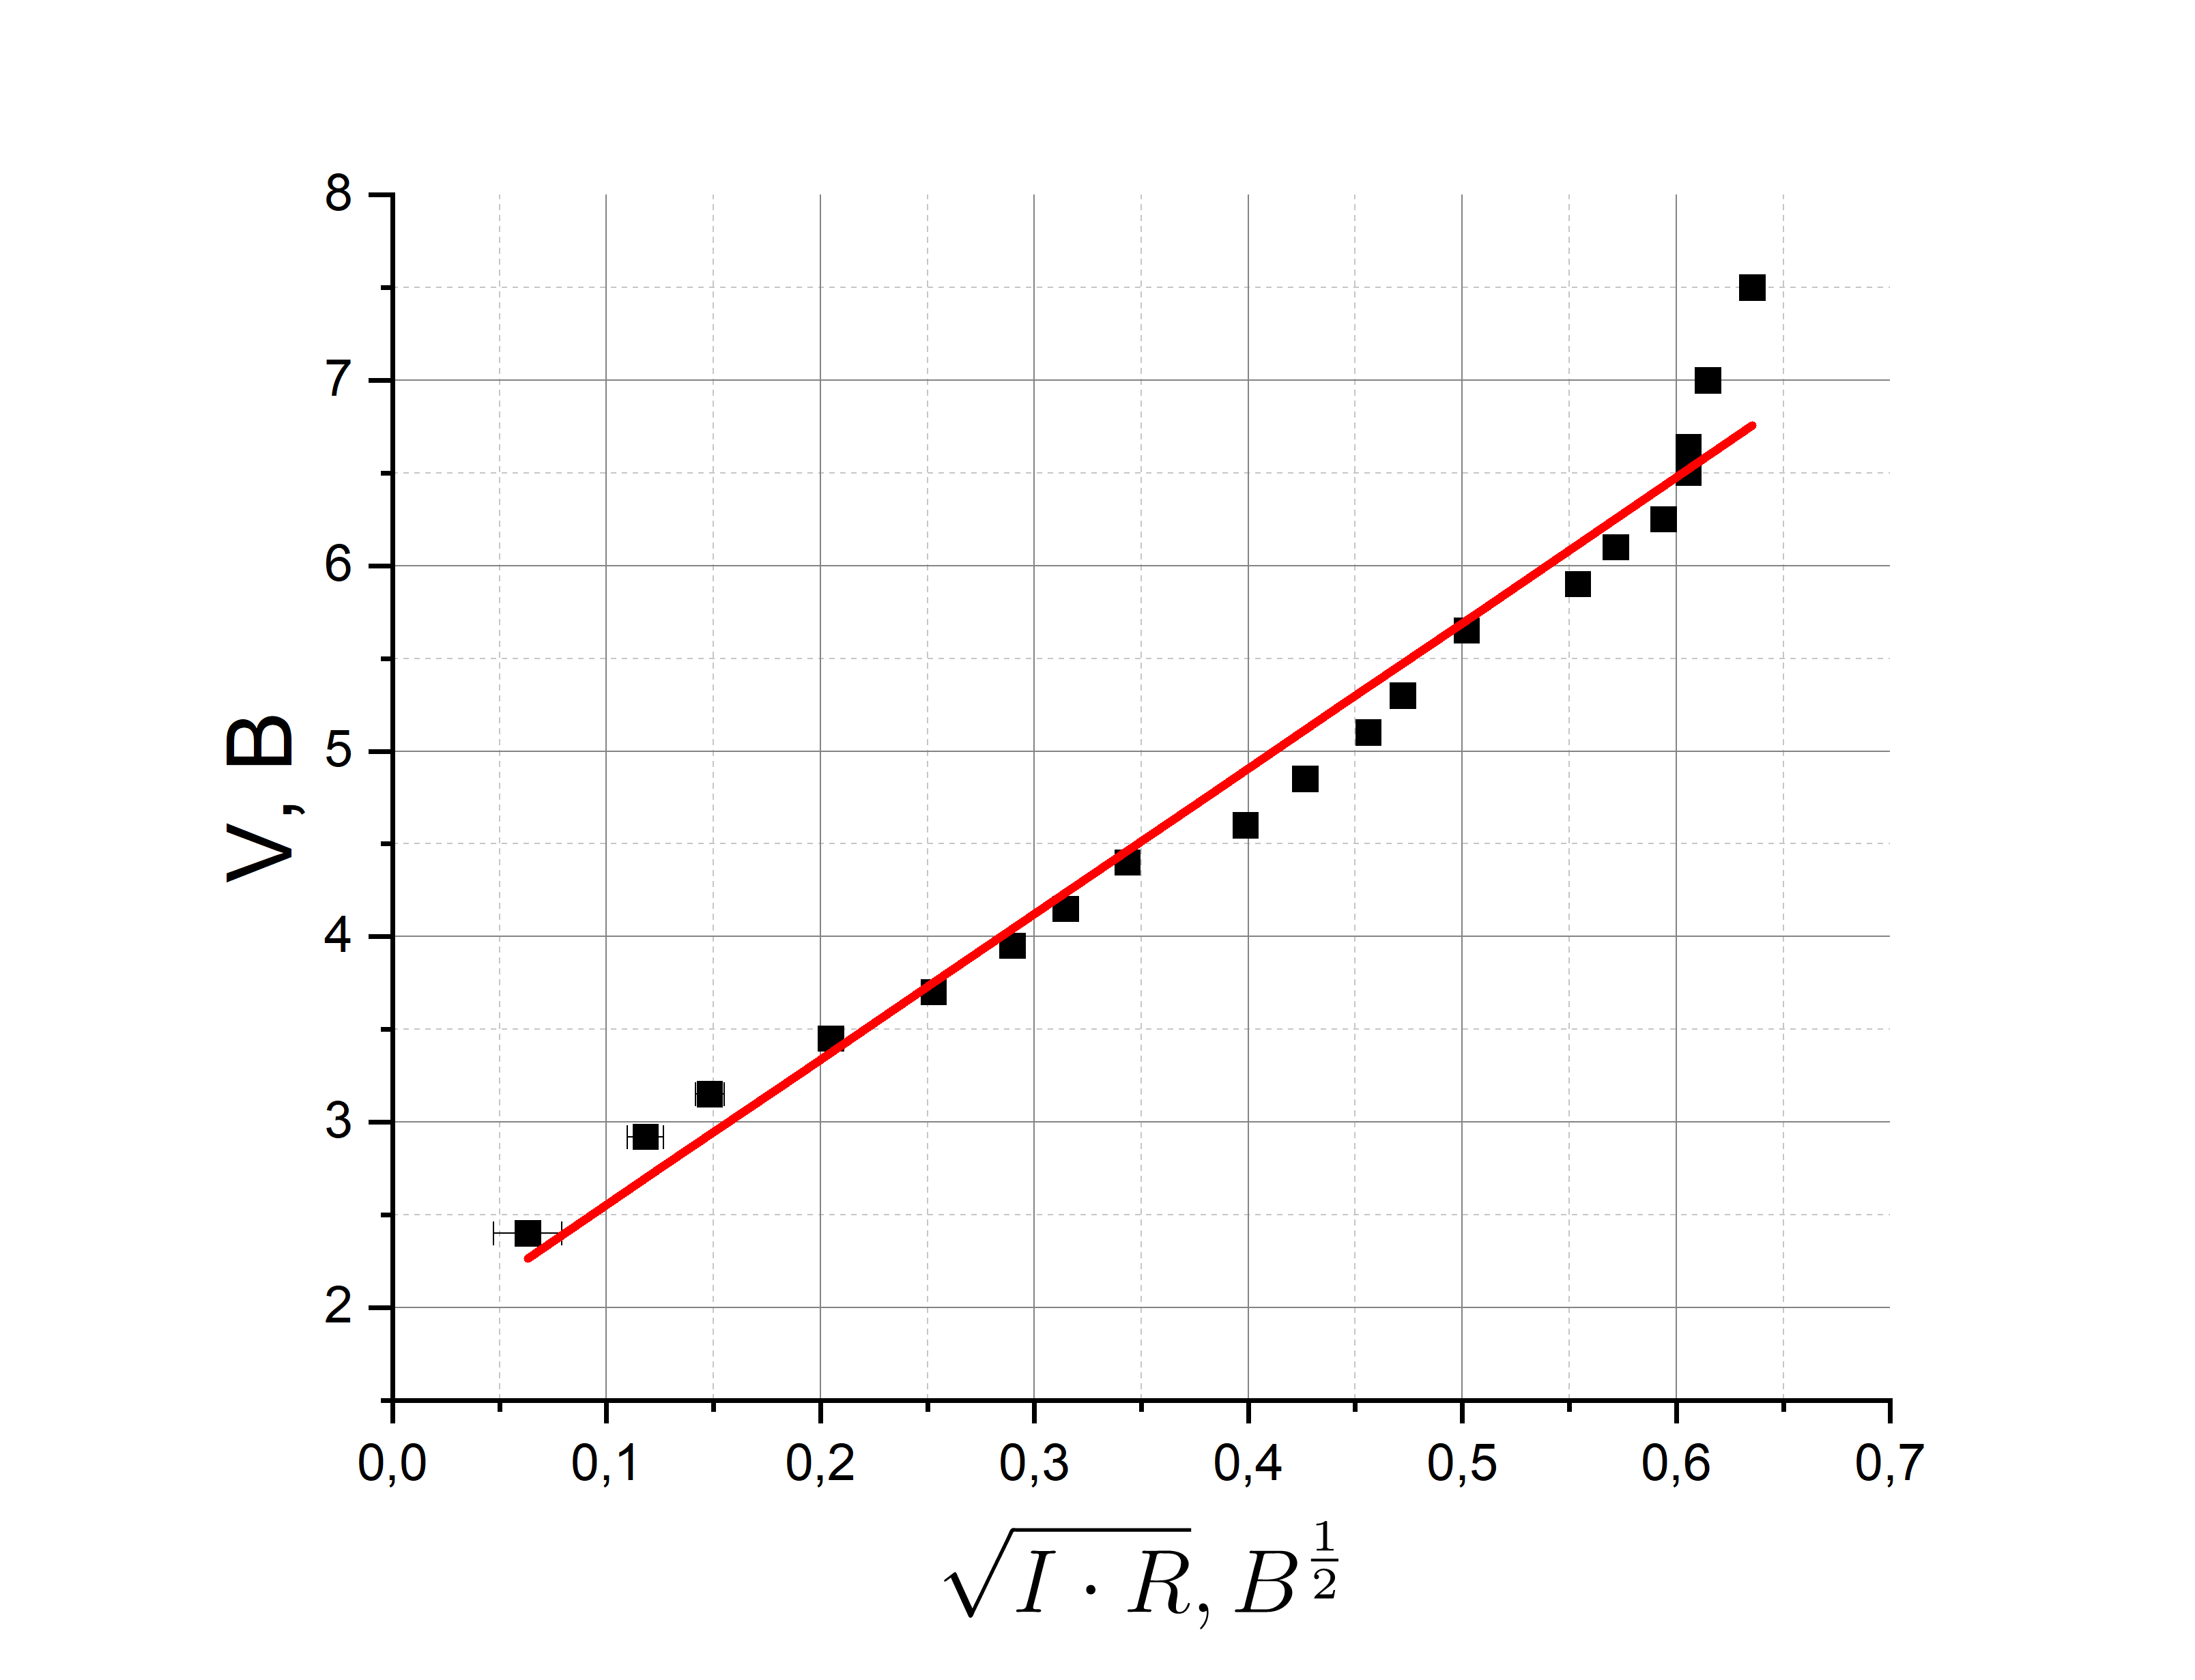
\includegraphics[width =0.8\linewidth]{lambda = 6939 A}
	\caption{График зависимости $f(\sqrt{IR}) = V$ для $\lambda = 6939 \ \mathring{A}$}
	\label{graph3:6939 A}
\end{figure}

\begin{figure}[h!]
	\centering
	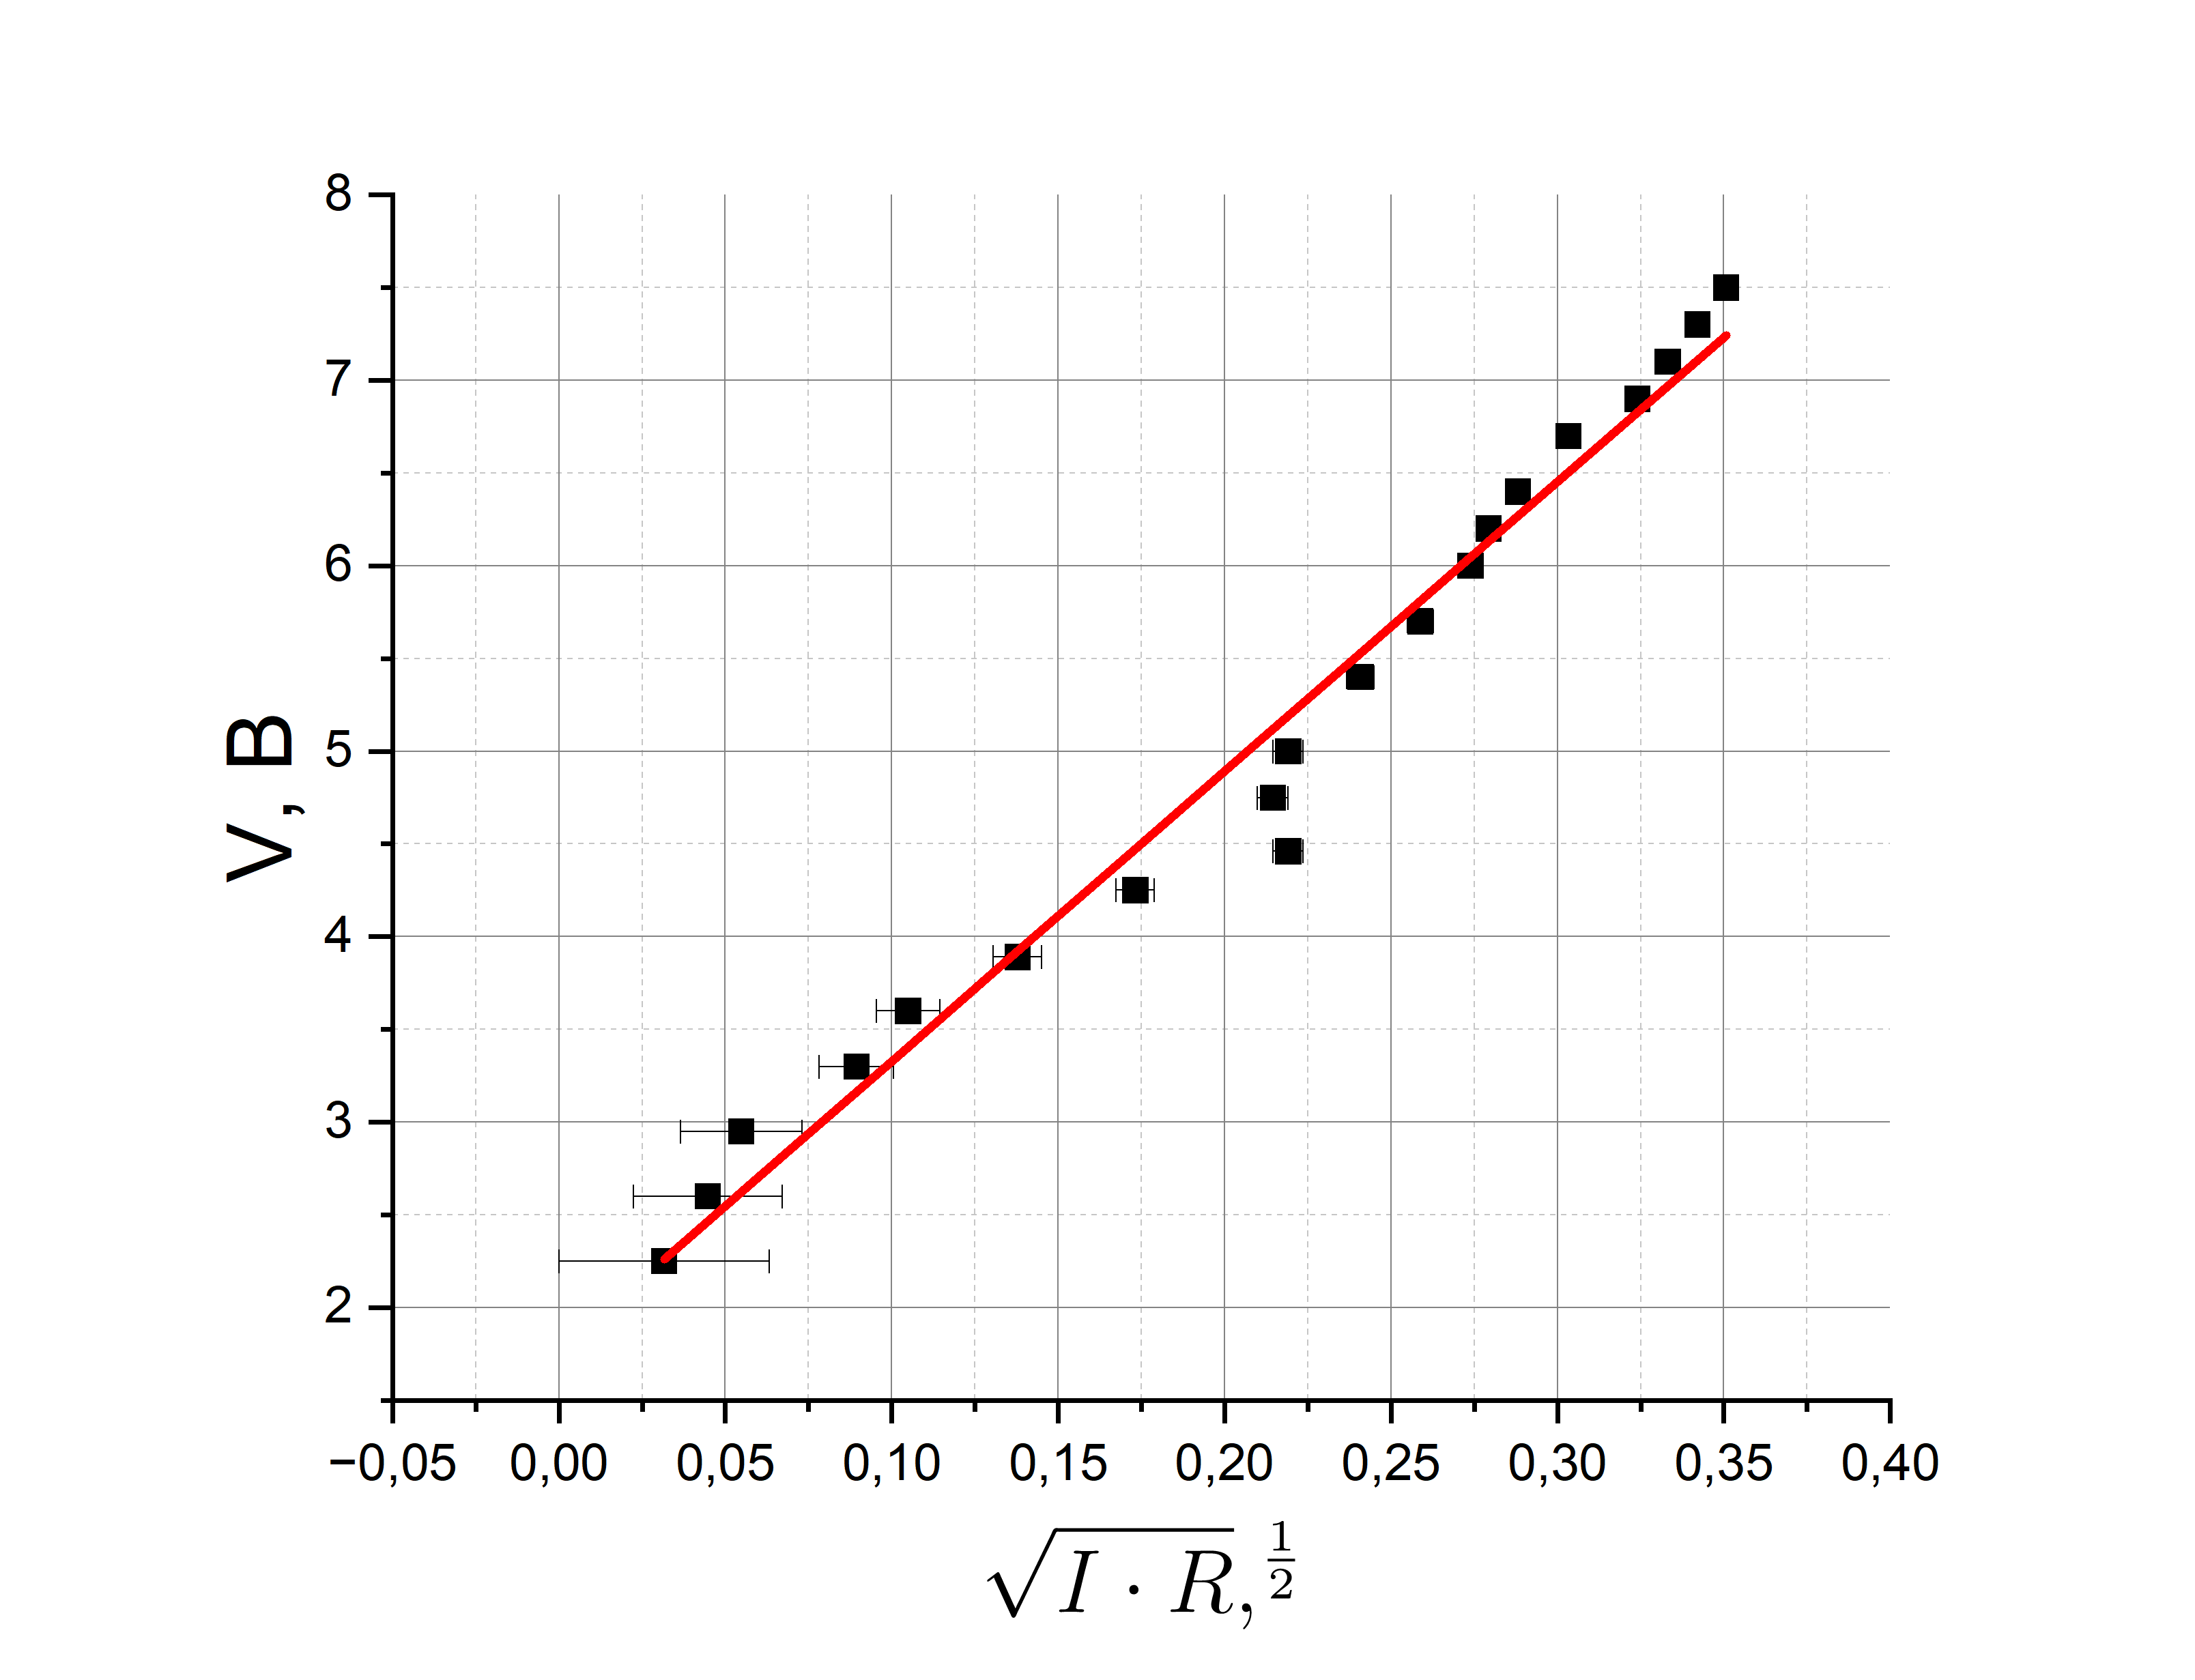
\includegraphics[width = 0.8\linewidth]{lambda = 6143 A}
	\caption{График зависимости $f(\sqrt{IR}) = V$ для $\lambda = 6143 \ \mathring{A}$}
	\label{graph4:6143 A}
\end{figure}

\pagebreak

\begin{figure}[h!]
	\centering
	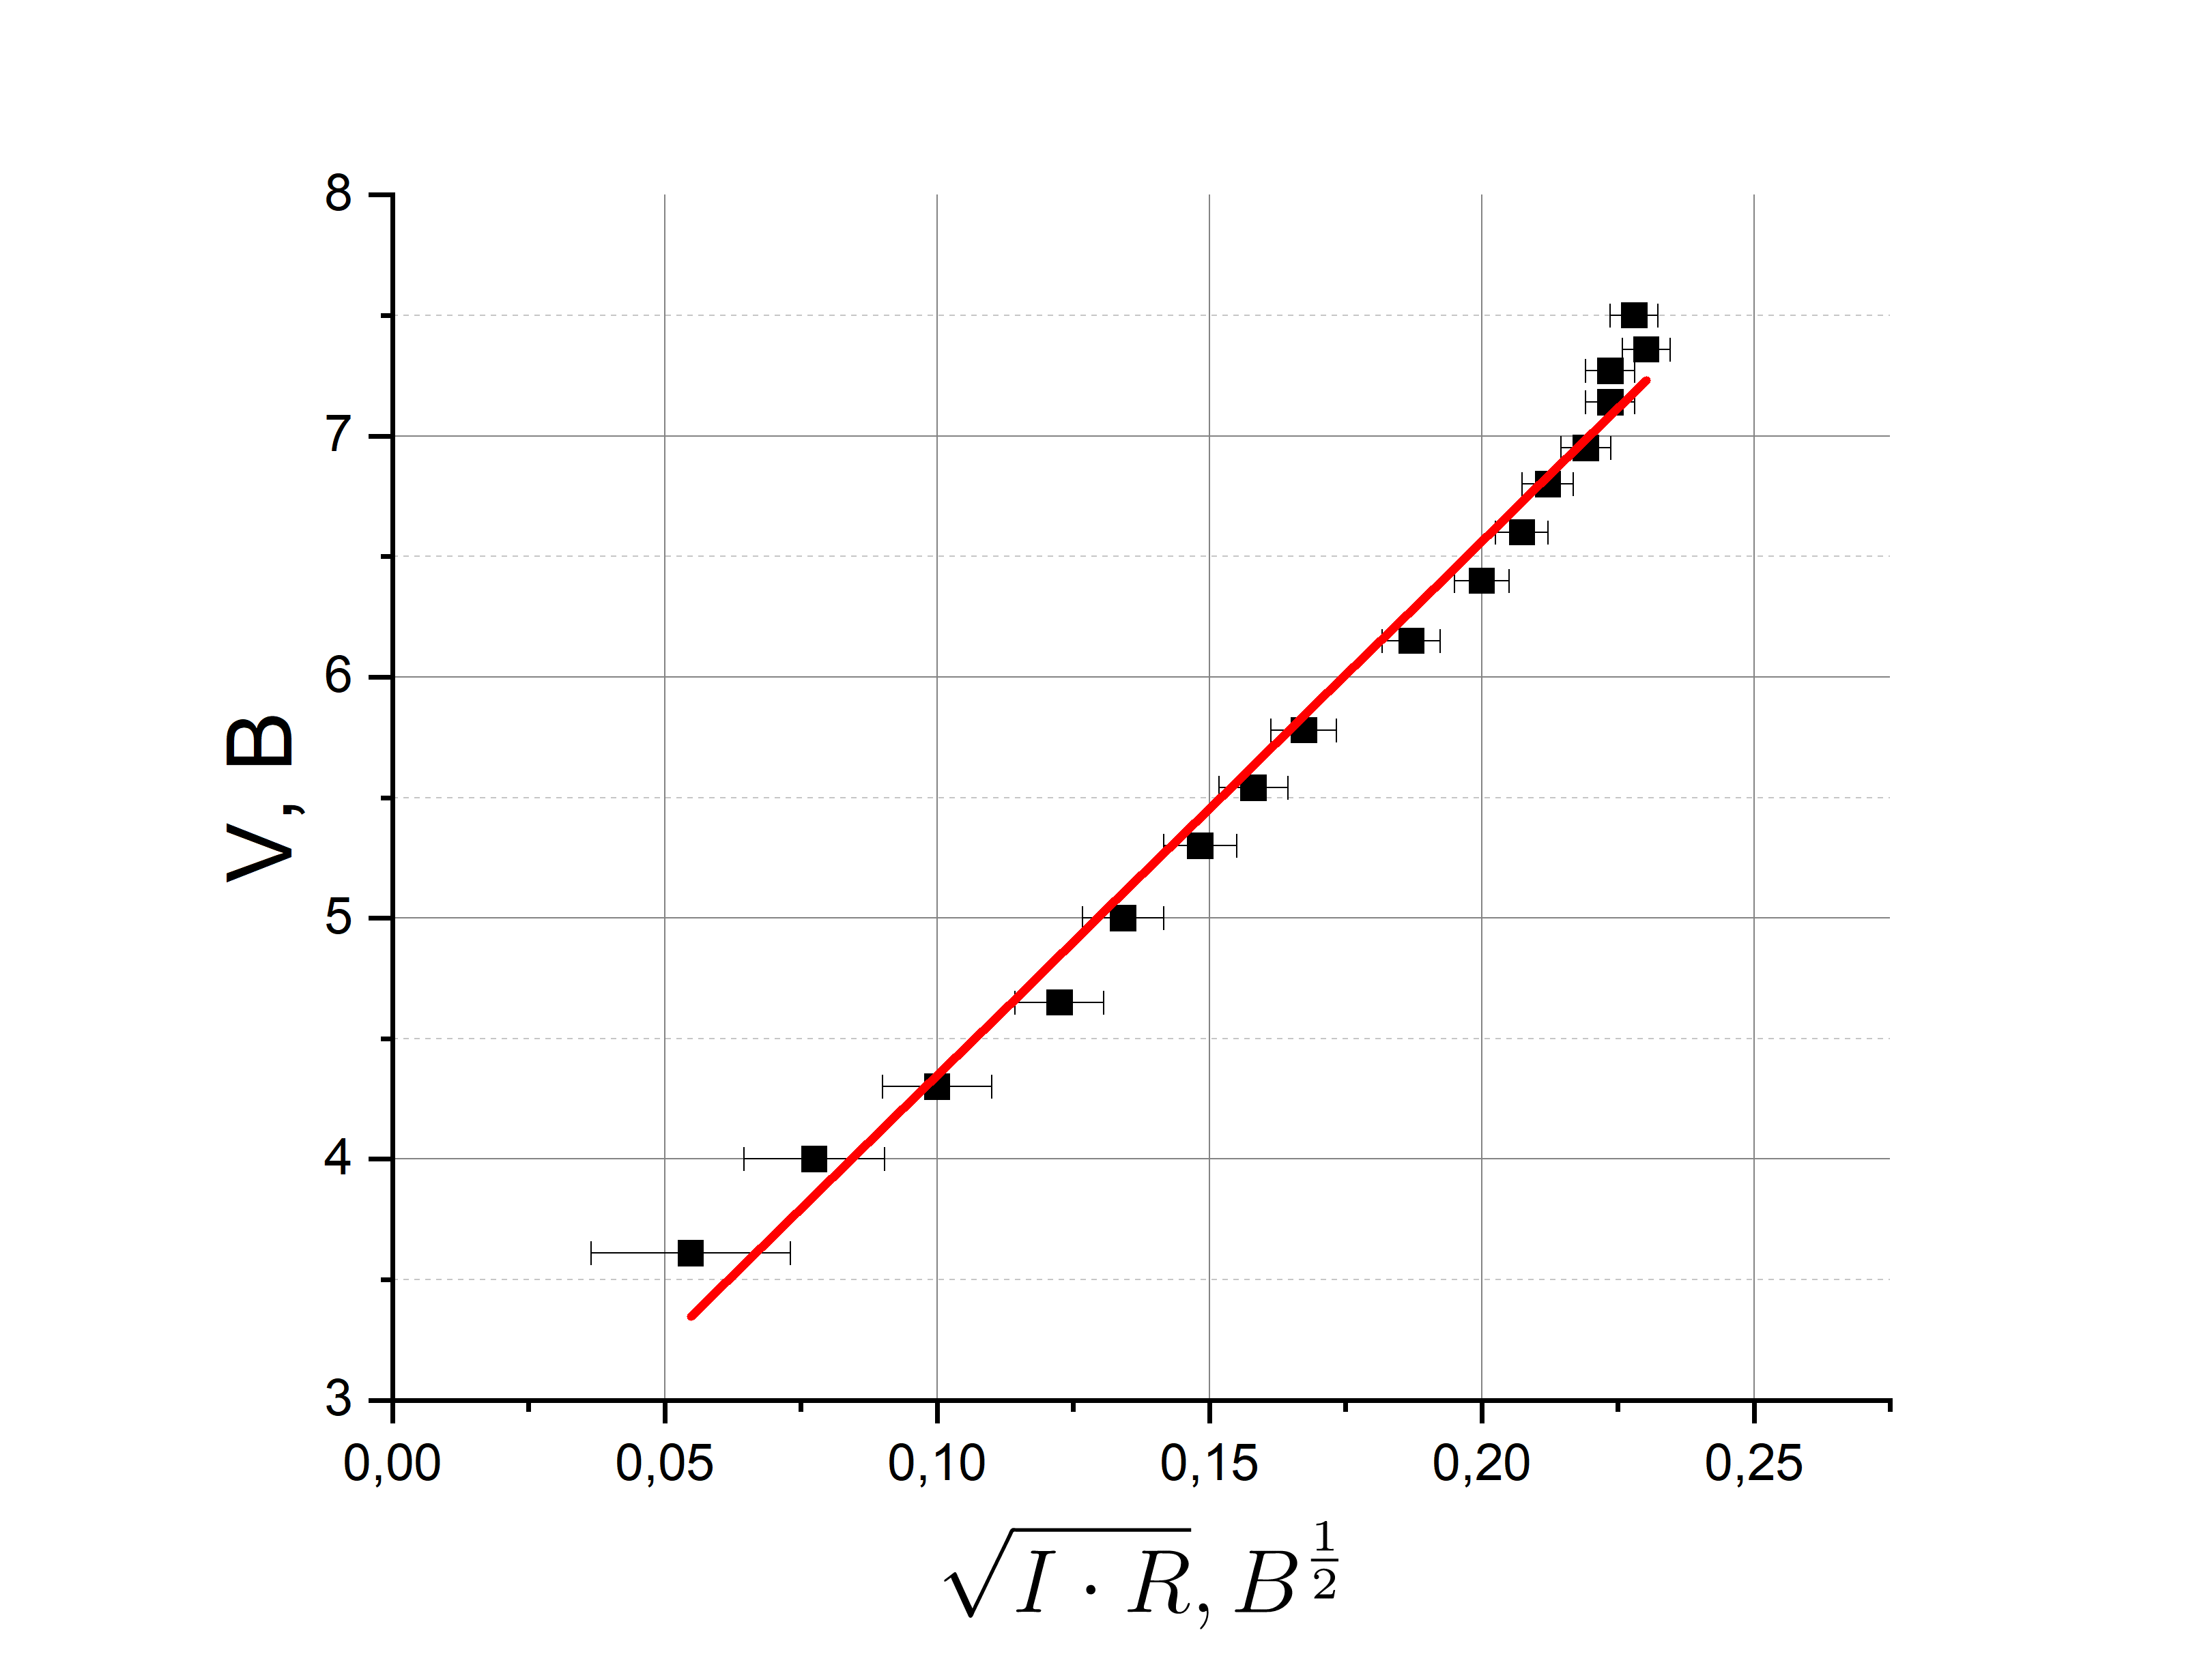
\includegraphics[width = 0.8\linewidth]{lambda = 5852 A}
	\caption{График зависимости $f(\sqrt{IR}) = V$ для $\lambda = 5852 \ \mathring{A}$}
	\label{graph4:5852 A}
\end{figure}

\begin{figure}[h!]
	\centering
	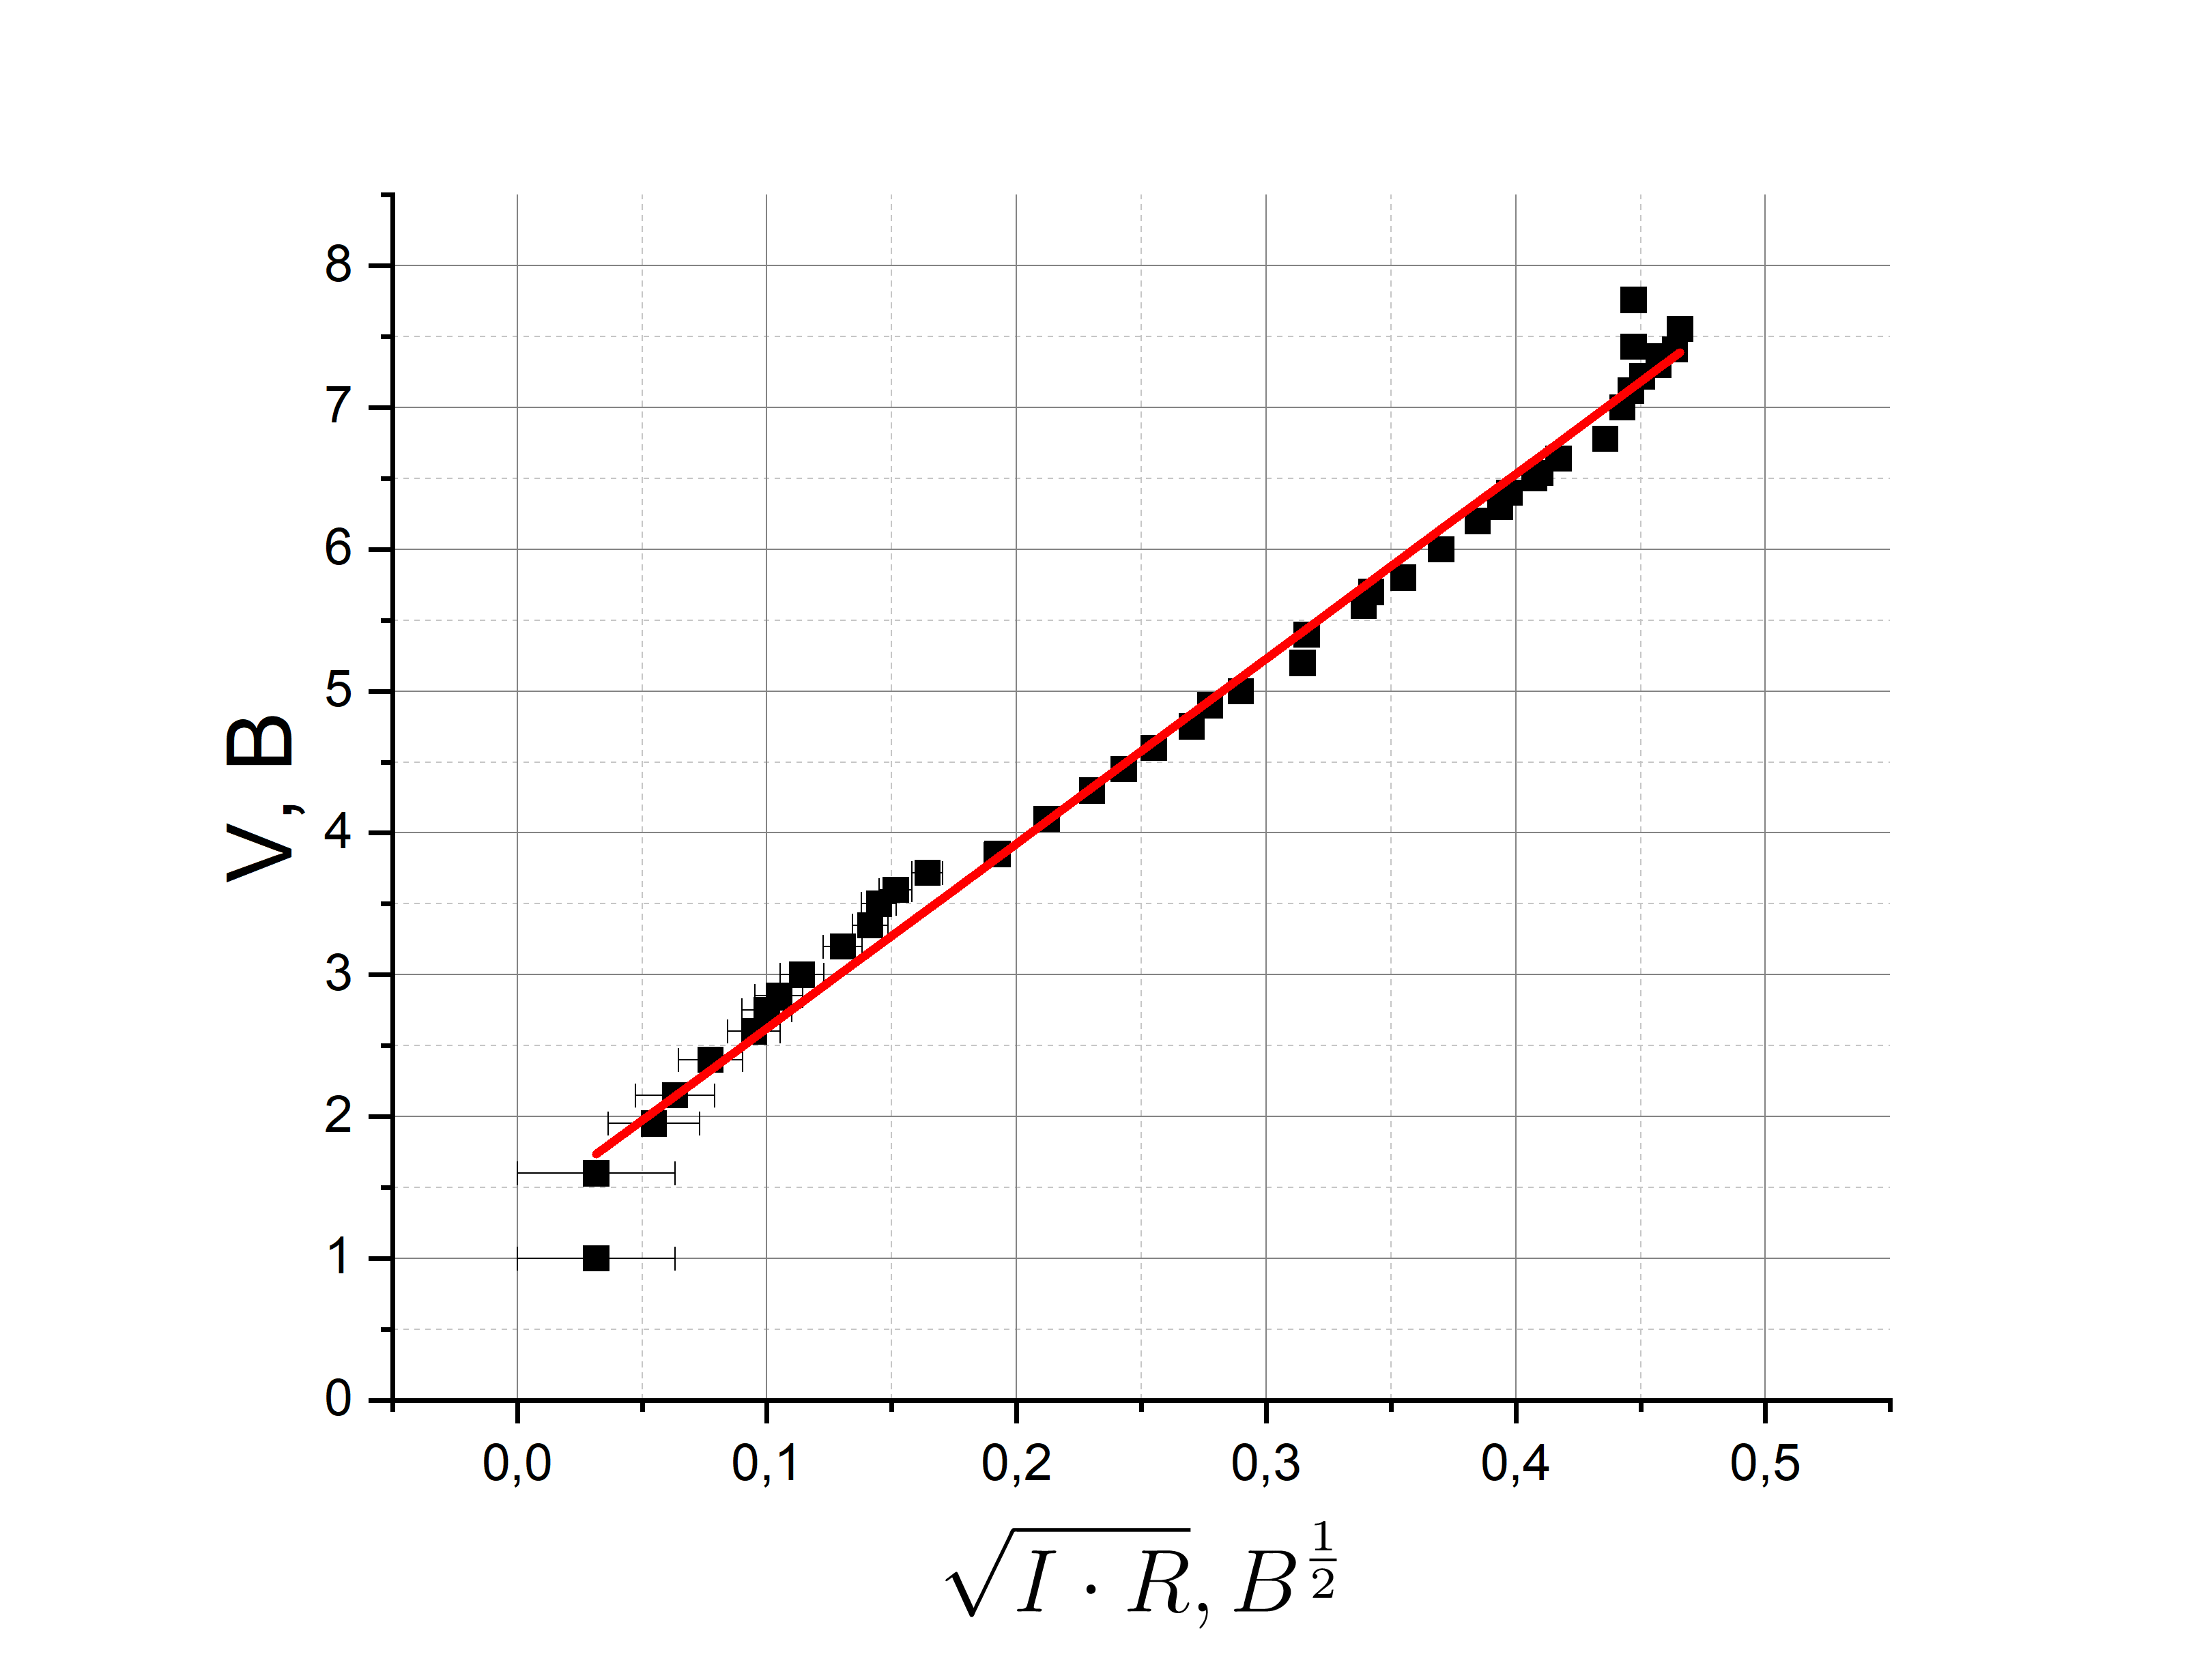
\includegraphics[width = 0.8\linewidth]{lambda = 5331 A}
	\caption{График зависимости $f(\sqrt{IR}) = V$ для $\lambda = 5331 \ \mathring{A}$}
	\label{graph5:5331 A}
\end{figure}

\pagebreak

Для каждой длины волны определим запирающее напряжение. Данные занесем в Таблицу \ref{table1:voltage}

\begin{table}[h!]
\centering
\caption{Запирающее напряжения для различных длин волн}
\begin{tabular}{|l|l|l|l|l|}
\hline
$\lambda, \mathring A$ & $6939$ & $6143$ & $5852$ & $5331$ \\ \hline
$V_0, В$ & $1,77 \pm 0,15$ & $1,77 \pm 0,13	$ & $2,13 \pm 0,13$ & $1,32 \pm 0,07$ \\ \hline
\end{tabular}
\label{table1:voltage}
\end{table}

Теперь построим график зависимости $V_0(\omega)$

\begin{figure}[h!]
	\centering
	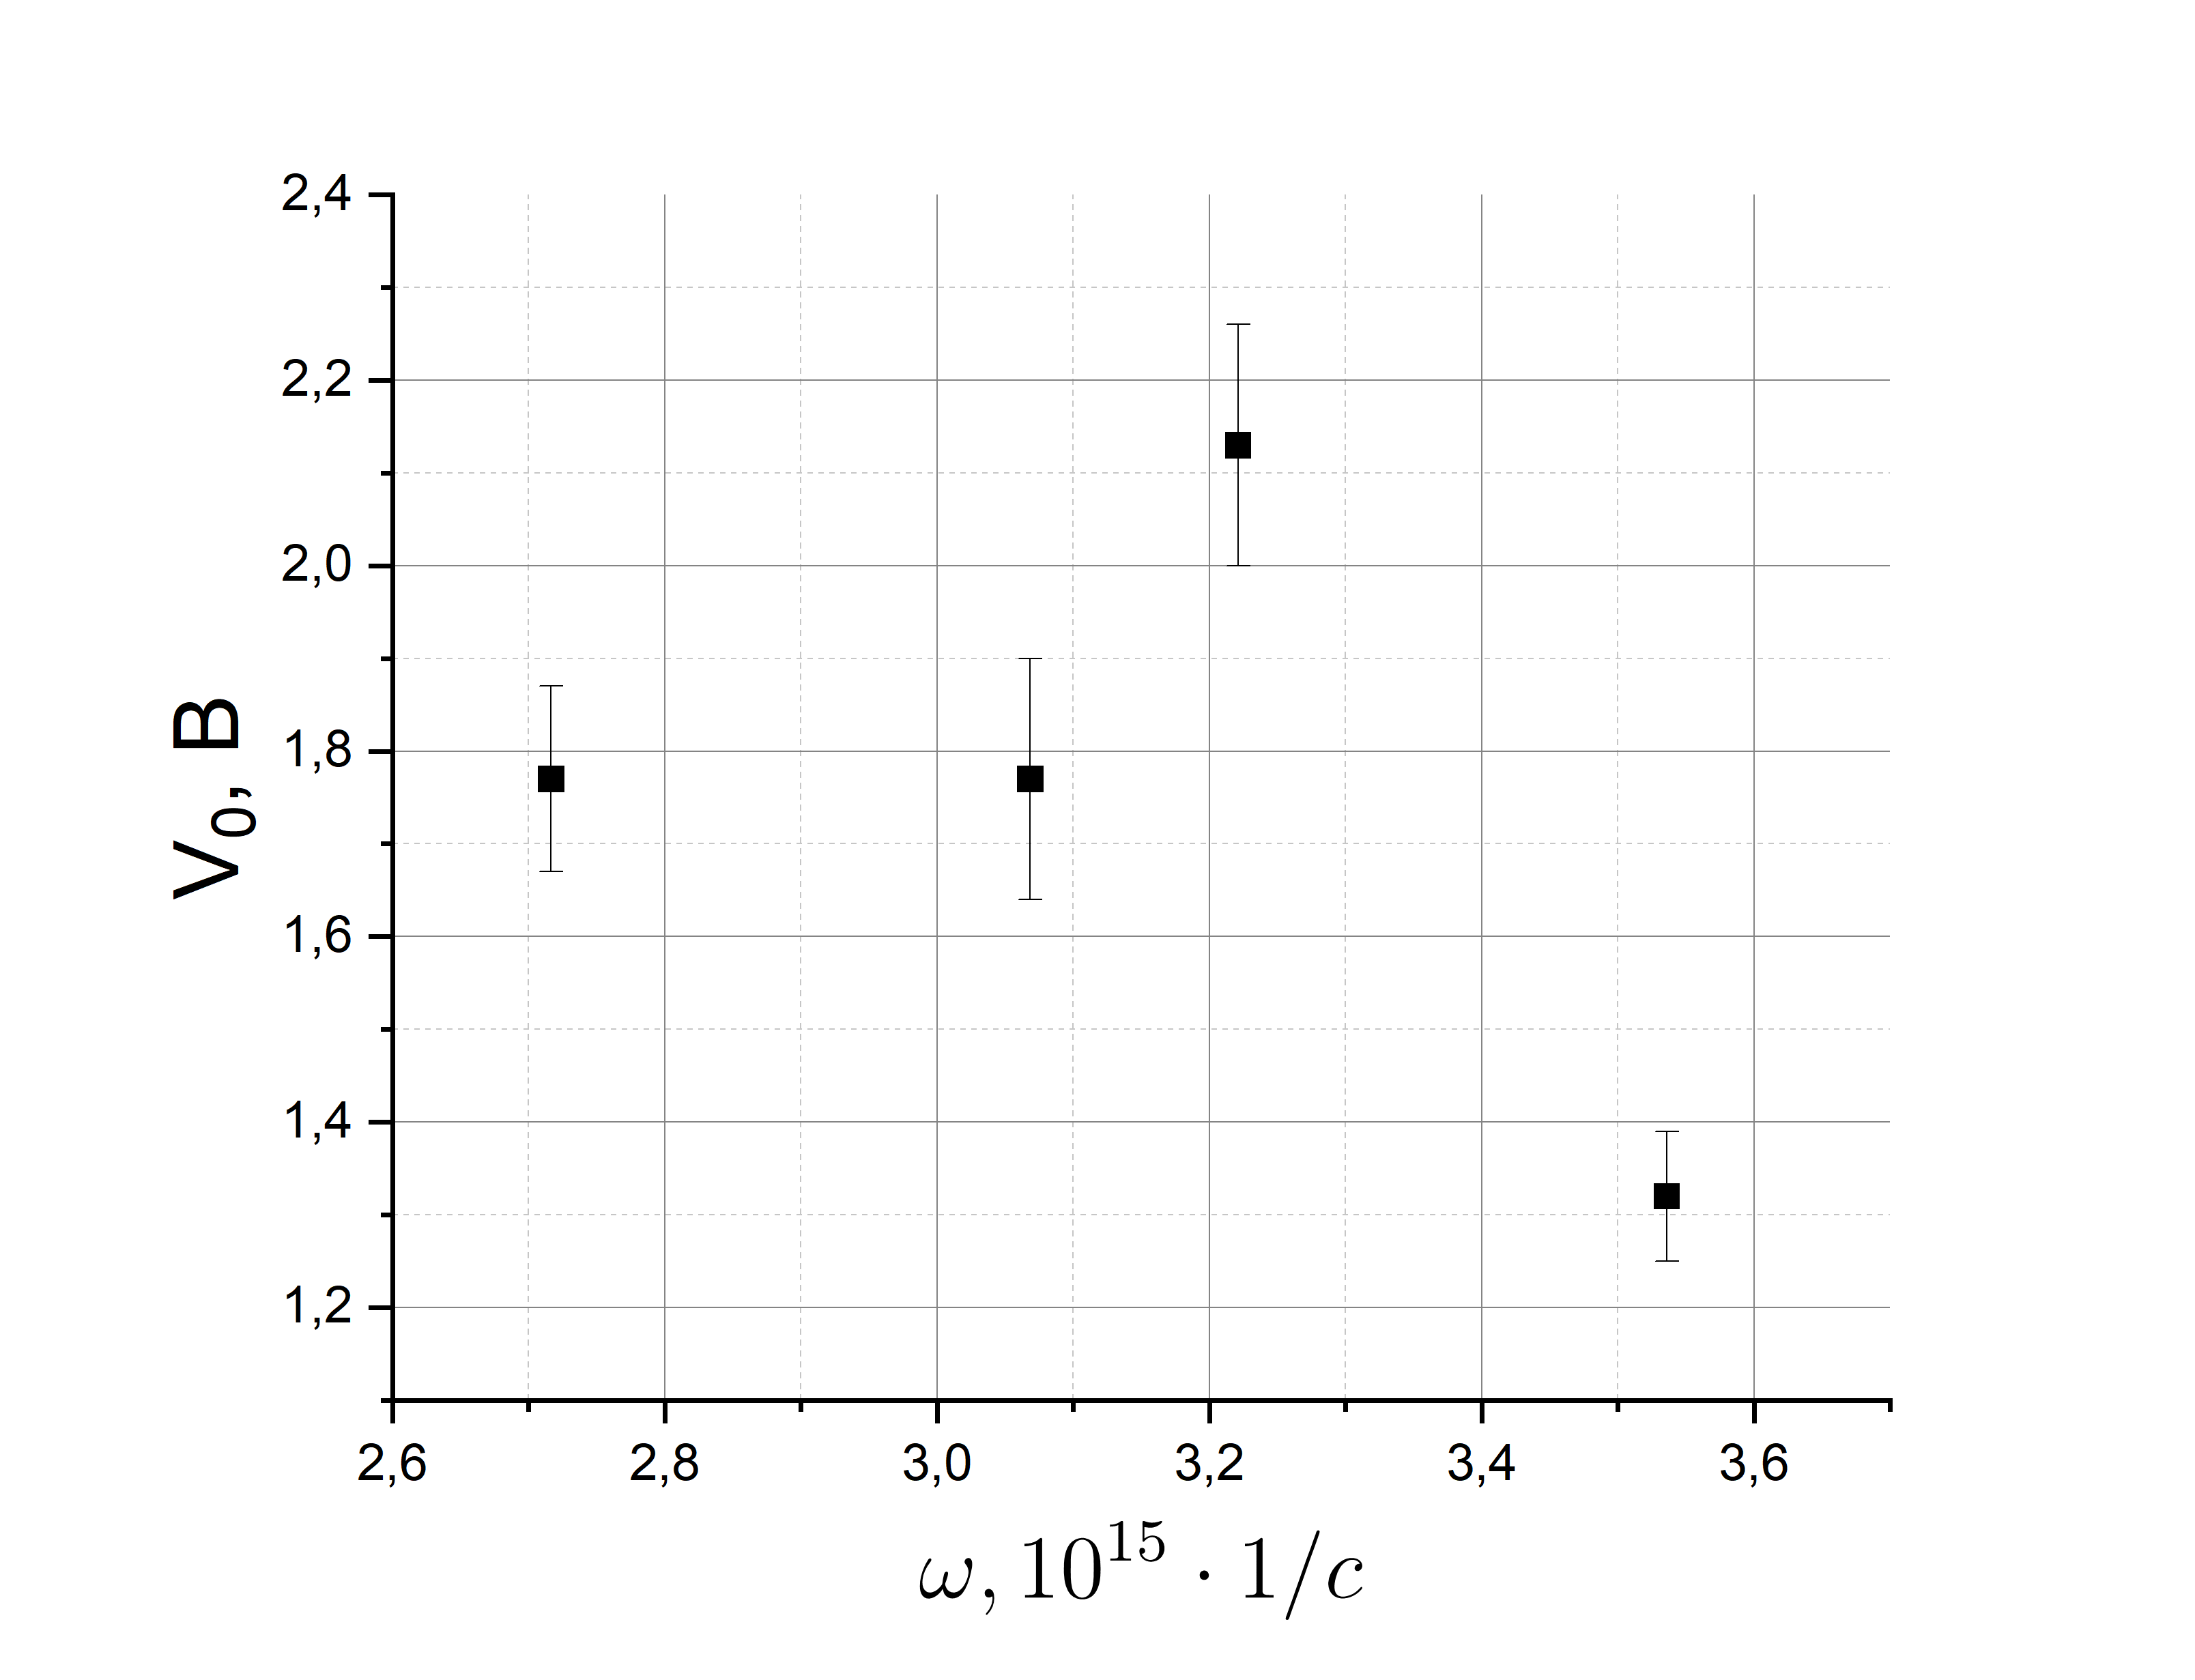
\includegraphics[width = 0.8\linewidth]{Stopping_voltage}
	\caption{График зависимости $V_0(\omega)$}
	\label{graph6:stop_voltage}
\end{figure}

Как видно из графика, точка, которой соответствует $V_0 = 1,32 В$, очевидно выбивается из линейной зависимости, это можно объяснить тем, что в середине измерений источник света <<съехал>> с исходного положения и большая часть света не попадала в монохроматор.

Отбросив данную точку аппроксимируем график:

\pagebreak

\begin{figure}[h!]
	\centering
	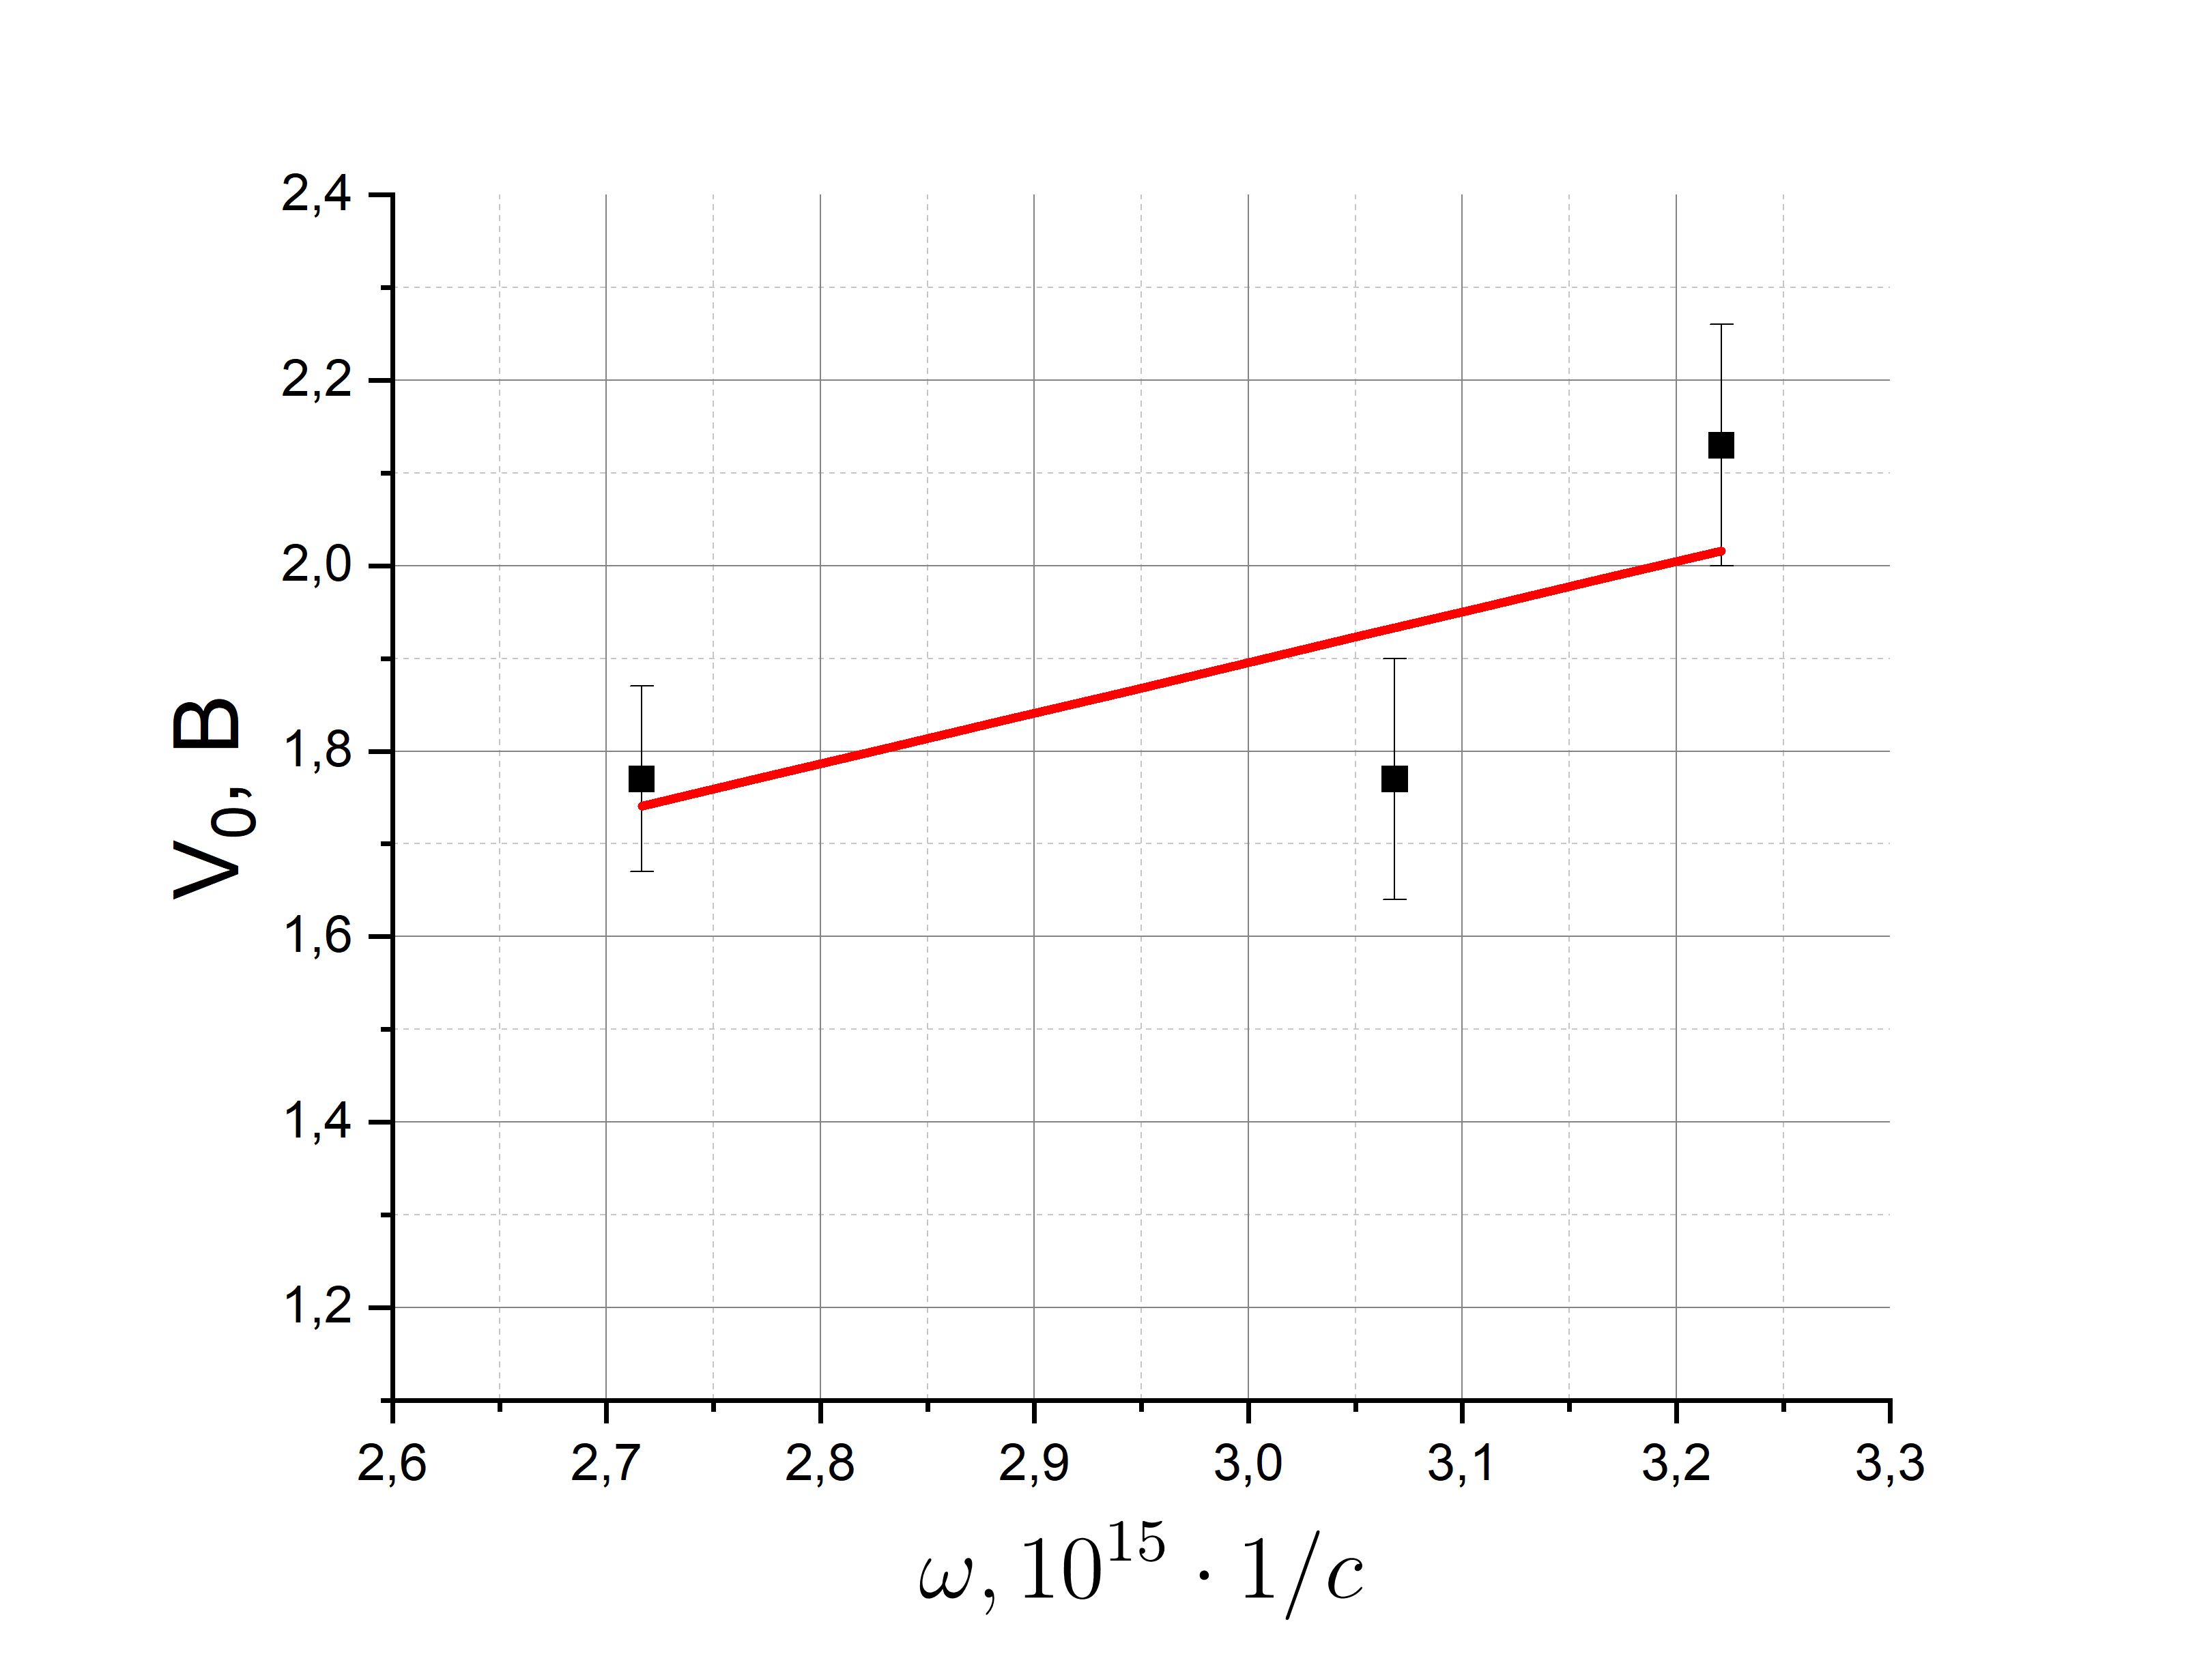
\includegraphics[width = 0.8\linewidth]{Stopping_voltage_2}
	\caption{График зависимости $V_0(\omega)$}
	\label{graph7:stop_voltage_2}
\end{figure}

Из аппроксимации:

$$
	\frac{dV_0}{d \omega} = ( 0,55 \pm 0,48 ) \cdot 10^{-15} \ В \cdot с
$$

Используя данное значение, оценим постоянную Планка:

$$
	\hbar = e \cdot \frac{dV_0}{d \omega} \approx (0,88 \pm 0,77) \cdot 10^{-34} Дж \cdot с	
$$

\section*{Выводы}

\begin{itemize}
	\item В результате работы, была получена экспериментально постоянная планка \linebreak $\hbar = (0,88 \pm 0,77) \cdot 10^{-34} Дж \cdot c$, что, в пределах погрешности, согласуется с теоретическими данными ($\hbar = 1,05 \cdot 10^{-34} Дж \cdot с$) 
\end{itemize}

\newpage

\section*{Приложение}

В заключении, приведем зависимости $\sqrt{I \cdot R} = f(V)$ для всех длин волн на одном графике

\begin{figure}[h!]
	\centering
	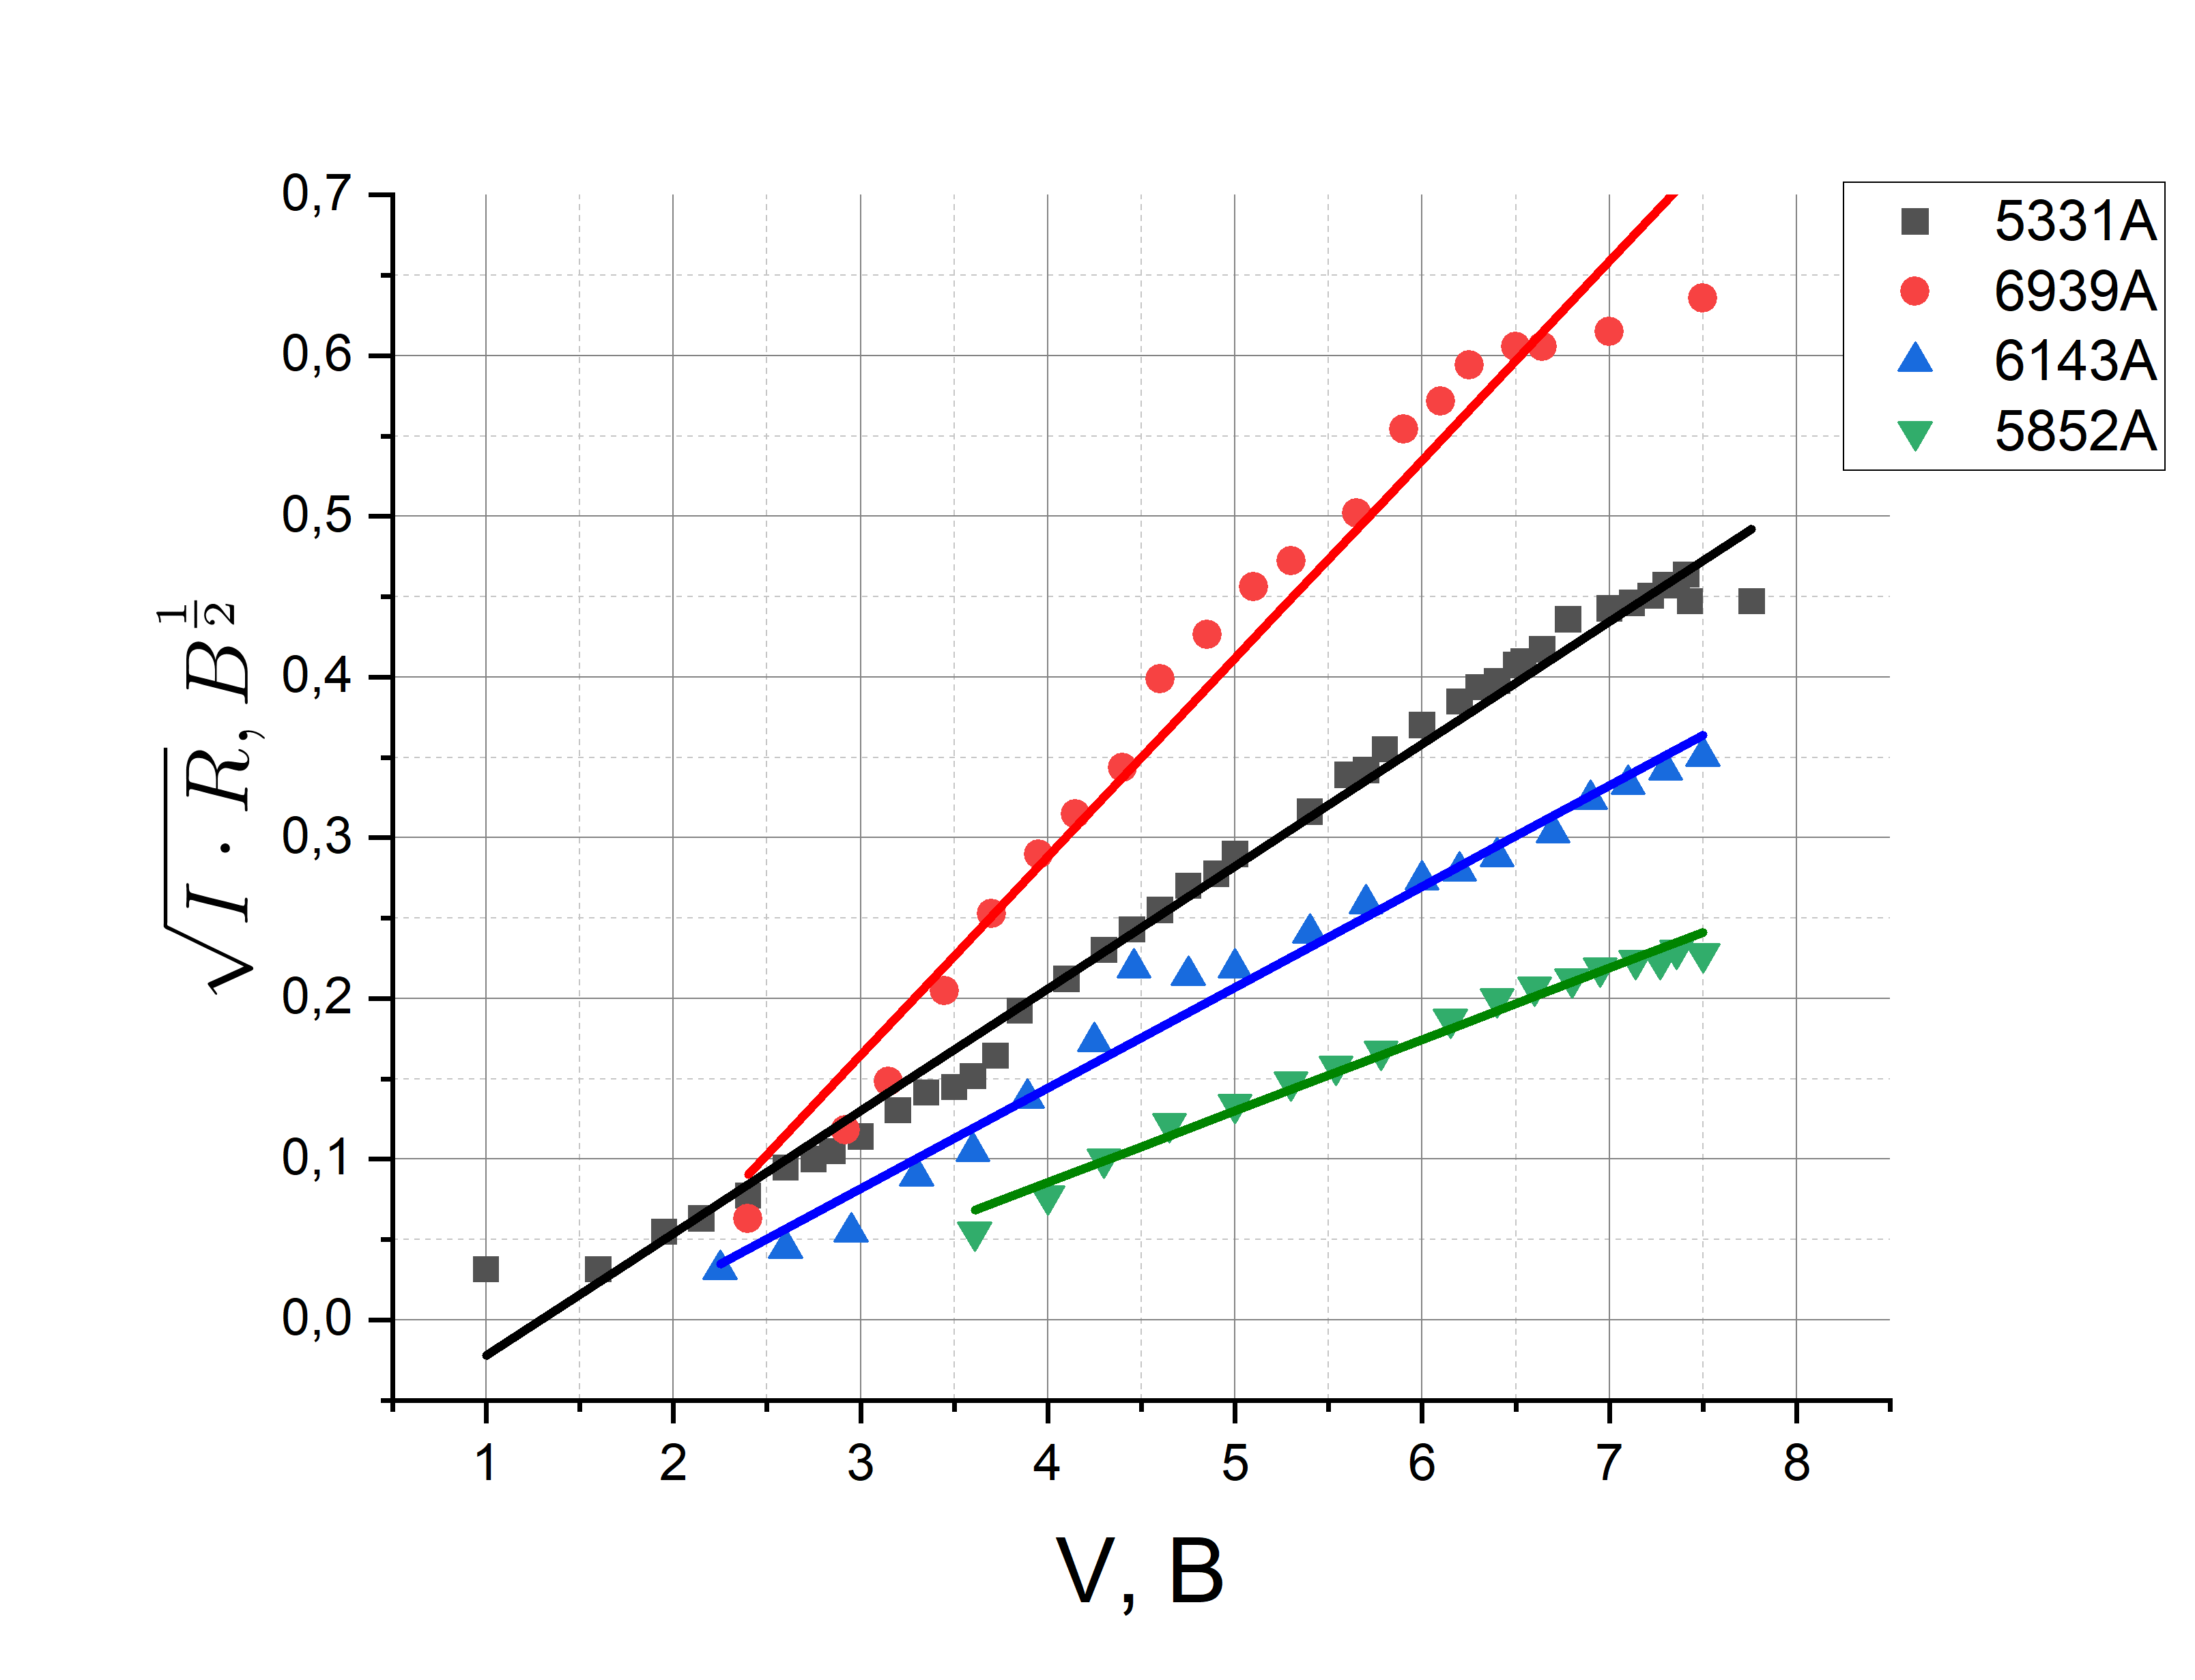
\includegraphics[width = \linewidth]{all_in_one}
	\caption{График зависимости $\sqrt{I \cdot R} = f(V)$ для всех длин волн}
\end{figure}


\end{document}
